\documentclass{article}
\usepackage{neurips_2024}
\usepackage{listings}
\usepackage{graphicx}
\usepackage[utf8]{inputenc} % allow utf-8 input
\usepackage[T1]{fontenc}    % use 8-bit T1 fonts
\usepackage{hyperref}       % hyperlinks
\usepackage{url}            % simple URL typesetting
\usepackage{booktabs}       % professional-quality tables
\usepackage{amsfonts}       % blackboard math symbols
\usepackage{nicefrac}       % compact symbols for 1/2, etc.
\usepackage{microtype}      % microtypography
\usepackage{xcolor}         % colors
\usepackage{natbib}
\usepackage{minted}
\usepackage{amsmath}
\usepackage{subcaption}
\usepackage{caption}


\title{ Hierarchical Transformation of Motor Representations: From Somatotopy to Functional Similarity in the Human Cortex}
\begin{document}
\maketitle


\begin{abstract}

The human motor system is traditionally understood through somatotopic maps like the motor homunculus, where neighboring brain regions control adjacent body parts. While this anatomical organization is well-characterized in primary motor cortex (M1), we've seen growing evidence that suggests higher-order motor areas may prioritize functional similarity—organizing movements by behavioral goals rather than physical proximity. Here, we systematically tested this hypothesis using high-resolution fMRI data from 62 participants performing 12 distinct body movements. We constructed representational dissimilarity matrices (RDMs) across four cortical regions—M1, SMA, PMC, and PPC—and compared them to two theoretical models: one based on anatomical adjacency and one on shared functional purpose. Representational similarity analysis (RSA) revealed a robust gradient: M1 aligned most strongly with anatomical organization, while SMA, PMC, and PPC showed progressively weaker anatomical fits and emerging functional structure. Multidimensional scaling (MDS) visualizations supported this transition, with higher-order regions exhibiting increasingly abstract representational geometries. Our results provide empirical evidence for a hierarchical transformation in motor representations, from effector-specific encoding in M1 to goal-directed codes in higher-order regions, offering new insight into the brain's organization of complex motor behavior.
\end{abstract}

\section{Introduction \& Background}

The organization of the motor system has long been described by the classical motor homunculus. This is a somatotopic map in which neighboring cortical regions correspond to adjacent body parts (\cite{penfield}). This topographic structure is especially prominent in the primary motor cortex (M1) and the primary somoatosensory cortex (S1), where different parts of the body are emphasized in different locations, with feet represented dorsally and face and mouth progressively represented ventrally (\cite{meier2008}; \cite{zeharia2012}). In fact, high-resolution neuroimaging has confirmed distinct, localized representations for even closely adjacent effectors, such as individual fingers \citep{ejaz2015}. Similarly, although in lower resolution, somatotopy has also been observed in the supplementary motor area (SMA) and the premotor cortex (PMC) (\cite{sma}; \citep{pmc}).

However, this anatomical account may oversimplify the brain's motor representation. An emerging body of work suggests that higher-order motor regions may increasingly encode movement information according to functional similarity rather than just anatomical adjacency. This has been defined in terms of the shared behavioral goals or co-occurrence statistics of movements. For example, neural activity patterns in the primary motor cortex reflect usage-based relationships among fingers more strongly than by their physical proximity \citep{ejaz2015}. This is consistent with motor interactions that facilitate coordinated, complex actions and are encoded in the parietal and premotor cortices \citep{Graziano2002}. Moreover, ultra-high-field imaging has uncovered networks in M1 that integrate both somatotopic and goal-related activity \citep{Gordon2023}.

This shift toward abstraction intensifies in higher motor regions. In SMA, PMC, and the posterior parietal cortex (PPC), neural representations generalize across effectors and emphasize action goals, such as reaching or grasping, over the specific limbs involved (\citep{Gallivan2013, turella2014, Filimon2009}). Furthermore, representations in these areas can remain stable across different effectors and even show overlap for anatomically distant yet functionally related body parts, such as the hand and mouth, supporting a more integrative and goal-oriented structure  \citep{Graziano2002} Thus while M1 retains strong anatomical mapping, higher-order motor regions show reduced somatotopy and increasing abstraction of movement representations (\citep{Gallivan2013}). Together, these findings point toward a hierarchical transformation in the motor system from concrete, effector-specific codes in early motor areas to abstract, goal-directed representations in higher-order regions. 

Despite this growing evidence, we still lack a systematic understanding of how these differing organizational principles are distributed across the motor hierarchy. The recent availability of high-resolution, whole-body somatomotor datasets presents a unique opportunity to evaluate these competing models of motor representation at scale (\cite{Donahue2018}).

This study aims to test whether different regions in the motor hierarchy organize movement representations based on anatomical proximity or functional similarity. Specifically, we assess whether cortical representations of body movements cluster by adjacency or by shared behavioral goals. To do so, we classify movements into pre-defined functional groups (in alignment with tasks performed by participants in the original experiment). By comparing representational structures across multiple cortical areas, we seek to identify whether (and where) a transformation from effector-specific to goal-directed representations occurs. These findings may provide insights into fundamental questions about how the brain organizes complex motor behavior and may reveal organizing principles that extend beyond classical homuncular mapping.


\section{Methods}
\subsection{fMRI Dataset}
\cite{Donahue2018} provide a full, high-resolution fMRI dataset for whole-body somatopic mapping. The authors present 2-mm isotropic resolution fMRI data from 68 healthy adult participants performing voluntary movements of 12 different body parts (see \ref{fig:og-exp} for exact experimental conditions). The task employed a block design with 16-second movement blocks interspersed with rest periods, totaling 6 functional runs of 7 minutes 44 seconds each. Following the principle of topographic organization of the cortical motor and sensory systems, the 12 movements were grouped into two sets to make the conditions for adjacent body parts into two sets (see \ref{fig:exp} for experimental paradigm). This reduced the overlap of BOLD signals from adjacent body parts and serves as a foundation for our definition of anatomical adjacency (see \ref{models}). The data can be accessed from the OpenNeuro public repository (accession number: \cite{data}). Although data is available for all 68 participants, the study excluded six participants from our analysis due to inferior performance during behavioral training, resulting in the final sample of 62 participants. We follow this criteria and perform the rest of our analysis on those 62 participants. 

This dataset offers several critical advantages for our present study. First, the 2mm isotropic resolution enabled precise delineation of subtle representational differences across motor cortical regions, which was essential for distinguishing between adjacent body part representations. Second, comprehensive spatial coverage extended throughout the cortex, cerebellum, and subcortical structures, providing the ability to examine multiple levels of the motor hierarchy simultaneously. Third, temporal signal-to-noise ratio (SNR) within primary sensorimotor regions was already robust in the raw preprocessed data and improved further after ICA-based denoising, which enhanced the separation of body part representations. Finally, the CIFTI format facilitated surface-based analyses that respected cortical topology while maintaining high spatial specificity, critical for mapping fine-grained somatopic organization. The study further confirmed head motion was in good control to accurately establish a topographic map of body movements. The authors show that brain activations for body parts that are far apart (e.g. finger vs tongue) are far apart in the brain, whereas body parts that are close together (i.e., finger vs wrist) are well separated but very close together in the brain, providing evidence for the motor homunculus representation of body parts in the brain. 

\subsection{Atlas-Based ROI Definition}
All analyses were performed on subject‑level GLM contrast maps that had been converted to CIFTI dscalar format using ciftify.  Because these files are expressed on the 91k grayordinate surface (HCP’s fs\_LR mesh), we adopted the Glasser HCP‑MMP 1.0 atlas, which is a surface‑based parcellation that assigns every cortical vertex to one of 379 defined parcels (\cite{atlas}). We chose this surface atlas as it avoided the dimensional mismatch that arises when volumetric masks are applied to CIFTI data and it ensured that each vertex was uniquely attributed to a parcel, simplifying ROI construction and cross‑subject alignment in our analysis. 

Using the MMP lookup table, we grouped atlas parcels into four cortical regions of interest (ROIs) that span the motor hierarchy: the primary motor cortex (M1), the supplementary motor cortex (SMA), the premotor cortex (PMC), and the posterial parietal corext (PPC). These four areas were chosen based on their established established roles in motor execution, planning, and sensorimotor integration as well as their relevance in related literature, allowing us to examine how representational structure varies along a functional hierarchy from effector-specific to more abstract representations.

The M1 comprised bilateral area 4 (L\_4, R\_4); the SMA comprised medial area 6 (L\_6\text{ma}, R\_6\text{ma}); the PMC combined lateral premotor subdivisions (L/R\_6\text{mp}, 6\text{d},6\text{v},6\text{r}); and the PPC combined superior‑parietal and intraparietal parcels (L/R\_7\text{Pm}, 7\text{m}, 7\text{Am}, 7\text{PL}, 7\text{PC}, L\text{IPv}, \text{VIP} , \text{MIP}). Parcel IDs were converted to binary vertex masks, yielding one surface mask per ROI.
 
\subsection{Theoretical Models}
\subsubsection{Anatomical Adjacency Model}
To quantify the traditional homunculus organization hypothesis, we developed an anatomical adjacency model determined through careful consideration of established neuroanatomical literature and previous somatotopic mapping studies
Our model assigns each body part a specific coordinate value reflecting its position along the established dorsal-ventral gradient of the primary motor cortex. For example, spacing between hand segments (finger: 4, wrist: 3.6, forearm: 3.3, upper arm: 3) reflects the cortical representation of upper limb effectors. Furthermore, the left and right legs receive closely adjacent coordinates (2 and 2.1, respectively) to account for their bilateral representation while maintaining their proximity. Thus under this model, relative distance between different body parts is defined by distance between their corresponding coordinates (see \ref{tab:coords}). (Note that although guided by existing literature, these values were arbitrarily chosen and refined iteratively. They are but one set of numbers that follow well-established dorsal-ventral gradient with appropriate relative magnitudes). 

\begin{table}[h]
\centering
\begin{tabular}{|l|c|}
\hline
\textbf{Body Part} & \textbf{Coordinate} \\
\hline
toe & 0 \\
ankle & 1 \\
leftleg & 2 \\
rightleg & 2.1 \\
finger & 4 \\
wrist & 3. 6 \\
forearm & 3.3 \\
upperarm & 3 \\
jaw & 5 \\
lip & 5.1 \\
tongue & 5.2 \\
eye & 5.5 \\
\hline
\end{tabular}
\caption{Body part to coordinate mapping}
\label{tab:coords}
\end{table}

We transformed body part coordinates into a representational dissimilarity matrix (RDM) following standard procedures in representational similarity analysis (RSA). We computed pairwise Euclidean distances between the one-dimensional anatomical coordinates assigned to each body part, then normalized the resulting distance matrix to a [0, 1] range. This normalization preserved relative spatial relationships while ensuring comparability across models. The final RDM served as a benchmark for evaluating anatomical organization across brain regions.

\subsubsection{Functional Similarity Models}\label{models}
Our functional similarity models represented a critical departure from traditional anatomical approaches, operationalizing our hypothesis that higher-order motor regions organize movement information according to functional outcomes rather than anatomical proximity. Motivated by previous findings suggesting that neural representations reflect shared behavioral goals and motor synergies beyond strict anatomical adjacency \citep{ejaz2015}, we constructed a series of functional similarity models emphasizing ethological purposes and coordinated motor use.

Initially, we explored multiple complementary functional grouping schemes to evaluate different hypotheses about motor organization, each highlighting distinct aspects of functional similarity. A base model categorized body parts into five broad functional groups derived from general ethological roles (see \ref{tab:grouped_first}). Subsequently, we developed additional models informed by specific theoretical considerations from existing literature. A task-based model organized effectors according to inferred biomechanical roles, such as precision and power (see \ref{tab:grouped_task}). A coordination-based model emphasized the anatomical synergies and co-occurrences involved in coordinated movement patterns (see \ref{tab:grouped_coord}). 

Ultimately, we selected the goal-oriented categorization as the primary functional model for our analysis. This model explicitly captured the behavioral objectives and outcomes served by different effectors, providing a nuanced representation of functional similarity based on shared ethological goals (see \ref{sec:future_work} for a more detailed analysis behind choice).

Like the coordination-based model, this goal-oriented scheme also incorporated dual membership, recognizing multifunctionality in effectors such as the forearm (participating in both hand complex and arm chain coordination \ref{tab:grouped_coord}) or the tongue (communication and ingestion \ref{tab:grouped_goal}).

To implement dual membership, our RDM construction algorithm calculated functional similarity based on category overlap. Two body parts were considered functionally similar if they shared at least one functional category, regardless of other category memberships. This binary approach assigned a similarity value of 0 if the parts shared at least one category and 1 if they belonged to entirely distinct groups, 
This captured functional similarity as a categorical distinction while accommodating the multifunctional nature of certain effectors, ultimately highlighting relevant organizational principles that might be obscured by
more rigid, singular categorization schemes.

The detailed functional categorization used in the goal-oriented model is shown in Table \ref{tab:grouped_goal} and is used for the rest of this paper. (Note that although this model provided refinement from our initial models, this is still only one of many groupings possible. Future work could explore group membership more closely) 

\begin{table}[h]
\centering
\begin{tabular}{|l|l|}
\hline
\textbf{Goal Category} & \textbf{Body Parts} \\
\hline
BALANCE & toe, ankle \\
LOCOMOTION & toe, ankle, leftleg, rightleg \\
MANIPULATION & finger, wrist \\
REACHING & forearm, upperarm \\
COMMUNICATION & jaw, lip, tongue \\
INGESTION & jaw, tongue \\
PERCEPTION & eye \\
\hline
\end{tabular}
\caption{Grouped body parts by shared movement goals}
\label{tab:grouped_goal}
\end{table}

\subsection{Theoretical Models}
Under our anatomical and functional models, we would expect dissociable patterns of representational similarity depending on the organizational principle present in a given brain region. If a region follows anatomical organization, we anticipate a graded pattern of dissimilarities corresponding to the spatial proximity of effectors on the motor strip. Thus movements involving nearby body parts (like wrist and forearm) should show higher similarity, while those involving distant effectors (toe and eye) should be maximally dissimilar (as reflected in the smooth gradient of the anatomical RDM Figure~\ref{fig:theoretical_rdms}, left). Conversely, if a region reflects functional organization, we expect sharp boundaries between functionally distinct groups, with high within-group similarity (zeros on the diagonal blocks) and maximal dissimilarity between groups, regardless of anatomical distance (as seen in the block structure of the functional RDM ~\ref{fig:theoretical_rdms}, right). These model predictions provide competing hypotheses for how motor representations are organized beyond primary motor cortex and offer a framework for interpreting empirical RDMs derived from neural data. 
\begin{figure}[!htbp]
\centering
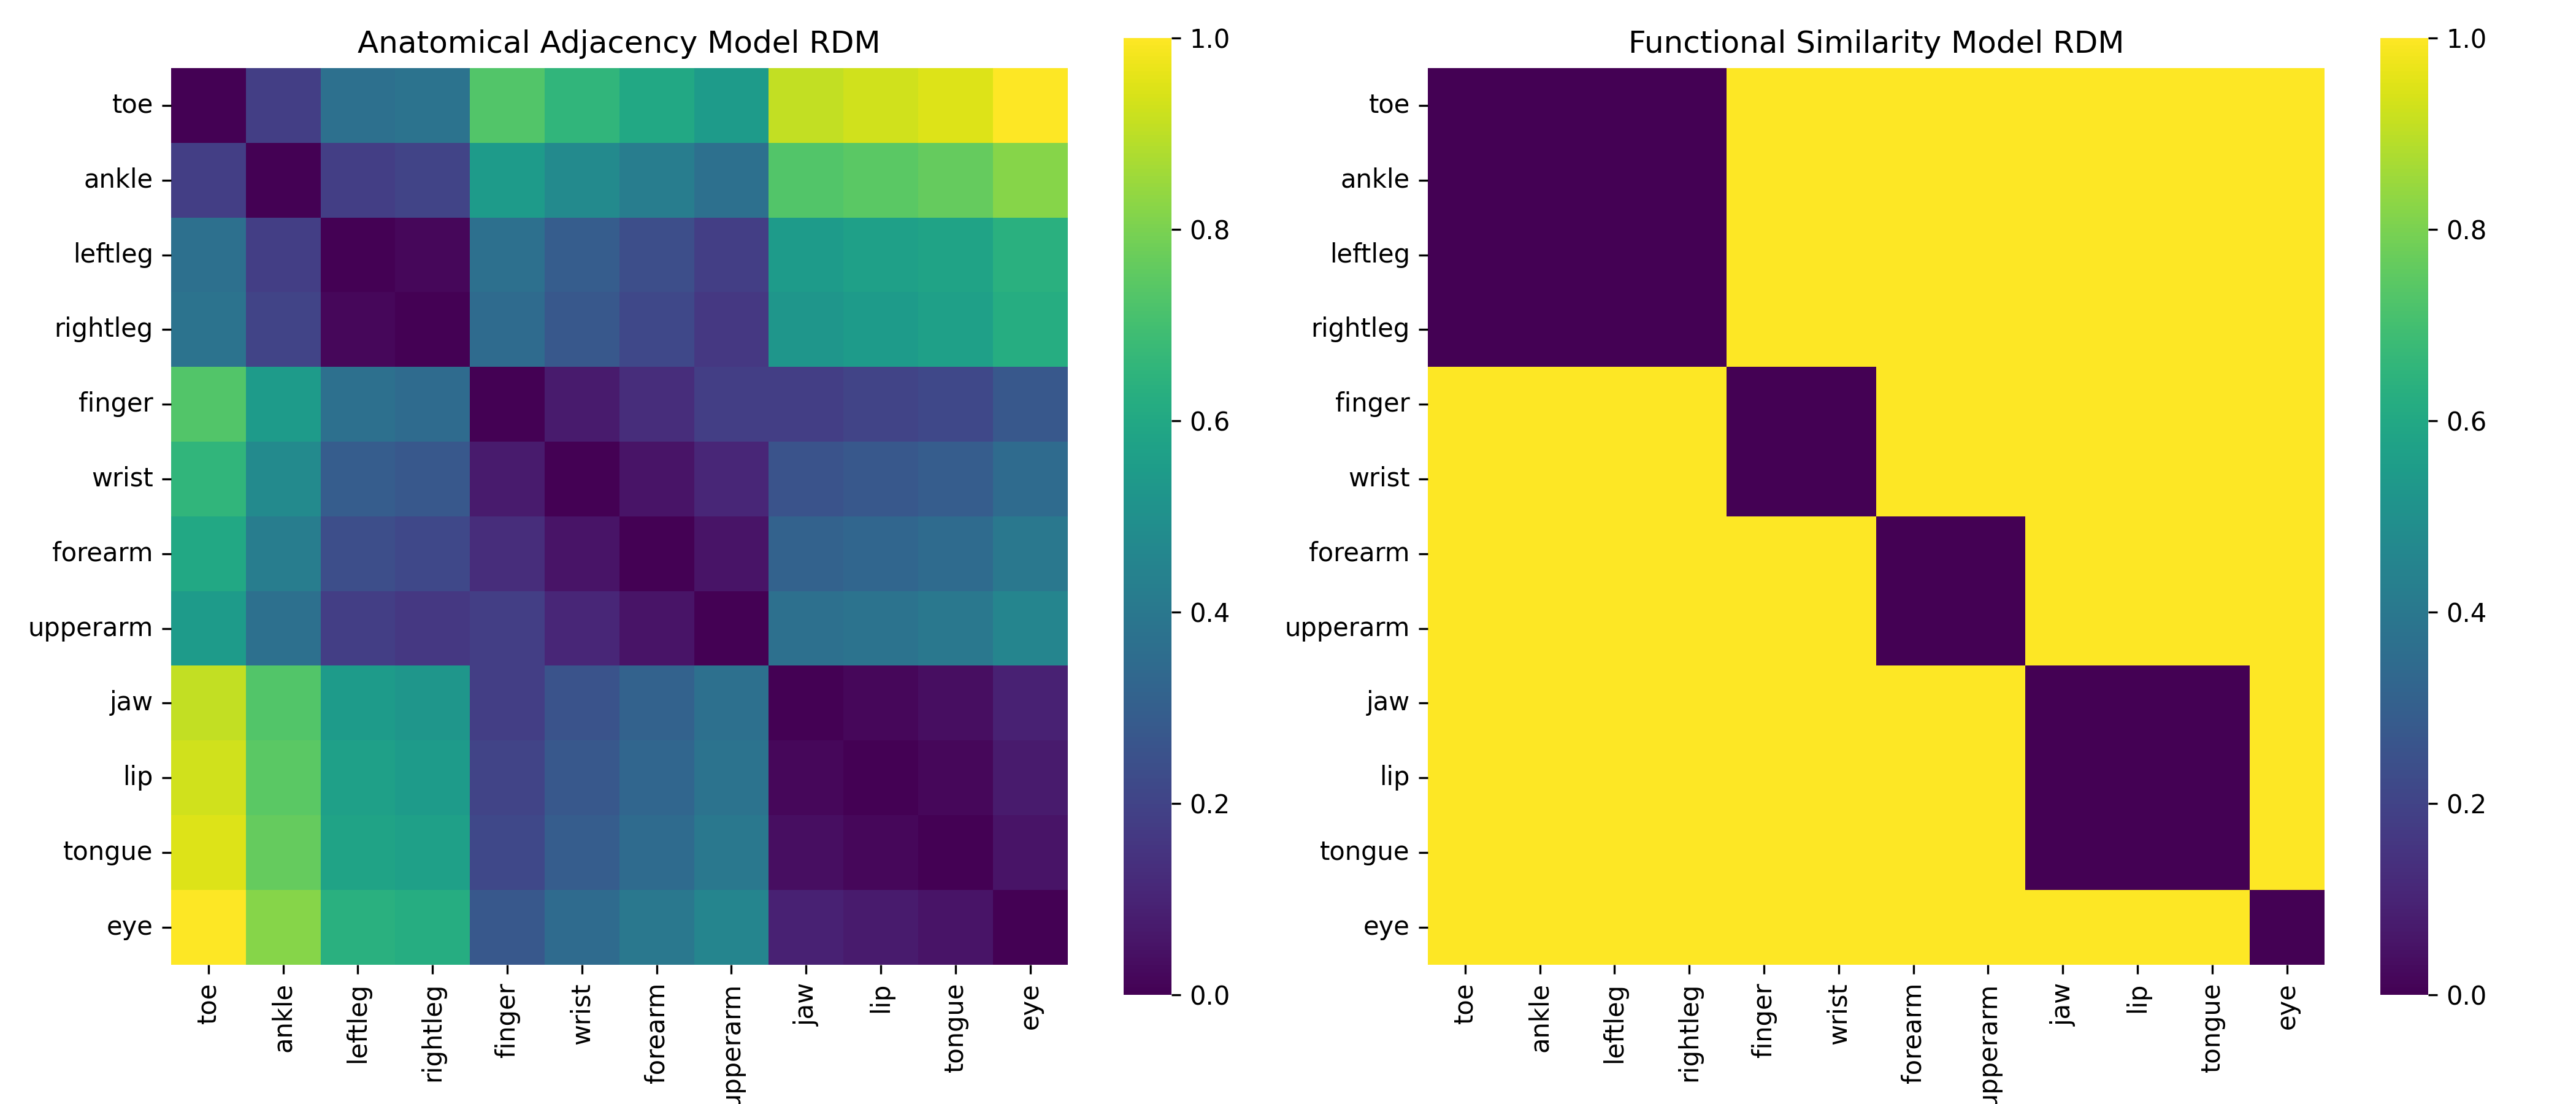
\includegraphics[width=0.8\textwidth]{results/goal_dual/theoretical_rdms.png}
\caption{Theoretical representational dissimilarity matrices (RDMs) for dual-goal functional categorization. Left: Anatomical Adjacency Model RDM shows graded dissimilarity based on spatial proximity. Right: Functional Similarity Model RDM shows discrete within-group similarity and sharp between-group dissimilarity.}
\label{fig:theoretical_rdms}
\end{figure}

\subsection{Pattern Extraction and RDM Computation}
We extracted body-part-specific activation patterns by applying each ROI mask to the subject-level general linear model (GLM) output in CIFTI dscalar format. These surface-based CIFTI files contained contrast maps for each of the 12 body part movement conditions. For each participant, we identified the corresponding contrast file for each condition and applied the ROI-specific grayordinate masks to isolate the pattern of activation values within each cortical region.

Each region x condition activation matrix was then standardized across vertices within each condition using z-scoring. This normalization step removed uninformative amplitude differences due to region-specific hemodynamic variability and ensured that representational similarity would reflect pattern shape rather than mean activation differences. After normalization, we computed pairwise Pearson correlation coefficients between all pairs of conditions to obtain a similarity matrix, and transformed this into a representational dissimilarity matrix (RDM) using $1-r$. This procedure was repeated for each subject and ROI, yielding a neural RDM per subject per region.

\subsection{Representational Similarity Analysis}
To test the alignment between neural representations and our two theoretical models, we performed representational similarity analysis (RSA) using rank-based (Spearman) correlations. Each subject-level neural RDM was compared to the anatomical adjacency and functional similarity model RDMs by computing the Spearman correlation between their upper triangular values (excluding the diagonal). This approach ensured a non-parametric, distribution-free measure of representational alignment and prevented redundancy from symmetric matrices.

By focusing on the upper triangle, we captured the 66 unique pairwise dissimilarities between the 12 body part conditions. These correlations served as our dependent measures for model fit in all subsequent analyses.

\subsection{Model Evaluation Across Subjects and ROIs}
We performed RSA for each of the 62 participants across the four ROIs (M1, SMA, PMC, PPC), generating two model fit scores (anatomical and functional) per subject per ROI. To evaluate group-level trends, we averaged the neural RDMs across subjects within each ROI and visualized these alongside the model RDMs as heatmaps.

% We then summarized model performance across ROIs by computing the mean and standard error of the RSA correlation scores across subjects. This summary enabled direct comparison of how well each model explained representational structure in each brain region. All results were stored in a structured dataframe and exported for reproducibility (and can be found in appendix).


\subsection{Model Comparison Framework}
We statistically compared the anatomical and functional model fits using paired-sample t-tests for each ROI. This approach accounted for within-subject dependencies, as each participant contributed both anatomical and functional RSA scores. By using paired tests, we maximized sensitivity to detect differences in model alignment without inflating the false positive rate.

We reported both t-values and p-values for each region. Where significant differences emerged, we determined which model provided a better fit by comparing group means.

\subsection{Hierarchical Organization Analysis}
To test our central hypothesis—that representational organization transitions from anatomical in M1 to functional in PPC, we computed difference scores between anatomical and functional RSA correlations for each subject. These scores were then aggregated by ROI and plotted in anatomical order (M1 $\rightarrow$ SMA $\rightarrow$ PMC $\rightarrow$ PPC). Positive difference scores indicated stronger anatomical alignment; negative scores indicated stronger functional alignment.

This analysis allowed us to assess whether a hierarchical gradient in representational format emerged across the motor control pathway, supporting theories of increasingly abstract movement representations in higher-order areas.

\subsection{Visualization Methods}
To visualize the structure of neural representations, we applied multidimensional scaling (MDS) to the average RDMs from each ROI. MDS projected the high-dimensional dissimilarity data into a two-dimensional space, where spatial proximity reflected similarity of body part representations. Points were color-coded based on functional group membership, enabling visual assessment of whether functionally similar movements clustered together. 

To supplement our visual MDS analysis with quantitative metrics of how `close' the projections aligned with our theoretical functional/anatomical models, we used Procrustes analysis to measure the similarity between empirical neural configurations and our theoretical models. Procrustes analysis then aligned these configurations by finding the optimal translation, rotation, and scaling transformations to minimize the sum of squared distances between corresponding points. This procedure generated a dissimilarity metric for each ROI-model comparison, which we converted to a similarity score (1 - dissimilarity) for intuitive interpretation, with values ranging from 0 (completely dissimilar) to 1 (identical configurations). We computed both anatomical and functional similarity scores for each ROI, as well as a functional dominance score (functional similarity minus anatomical similarity) to quantify the hypothesized transition from anatomical to functional representation across the motor hierarchy. We used these Procrustes metrics as an objective complement to visual inspection, so we could directly and numerically compare how closely each region's representational geometry adhered to our competing organizational models.

% Finally, we also created bar plots to summarize and compare RSA model fits, as well as a hierarchical plot illustrating the shift in model preference across regions. Together, these visualizations provided both quantitative and intuitive insights into how the brain organizes body movements.


% \subsection{Statistical Analysis}
% \subsubsection{Model Comparison Framework}
% We statistically compared the anatomical and functional model fits using paired-sample t-tests for each ROI. This approach accounted for within-subject dependencies, as each participant contributed both anatomical and functional RSA scores. By using paired tests, we maximized sensitivity to detect differences in model alignment without inflating the false positive rate.

% We reported both t-values and p-values for each region. Where significant differences emerged, we determined which model provided a better fit by comparing group means.

% To assess the robustness of our findings across different functional conceptualizations, we performed separate statistical analyses for each functional grouping approach (base functional, coordination-based, goal-oriented, and their dual-membership variants). This allowed us to evaluate whether our conclusions about hierarchical transformation were sensitive to specific functional definitions or represented a more general organizational principle across the motor system.

% \subsubsection{RSA Model Comparisons Across ROIs}
% To evaluate whether anatomical or functional models better explain the observed representational structures, we compared each neural RDM to both model RDMs using Spearman correlation. Results are summarized in Figure~\ref{fig:rsa}.

% Quantitative RSA revealed that the anatomical model consistently outperformed the functional model across all four ROIs (Figure~\ref{fig:rsa}). M1 demonstrated the strongest anatomical alignment (\(\rho = 0.600 \pm 0.015\)), significantly exceeding the functional model fit (\(\rho = 0.296 \pm 0.014\), \(t = 16.10\), \(p < .001\)). PMC showed a similar pattern (\(\rho_{\text{anatomical}} = 0.506\), \(\rho_{\text{functional}} = 0.296\), \(t = 9.72\), \(p < .001\)), as did PPC (\(\rho_{\text{anatomical}} = 0.340\), \(\rho_{\text{functional}} = 0.260\), \(t = 4.44\), \(p < .001\)). SMA also favored the anatomical model (\(\rho = 0.300\)) over the functional model (\(\rho = 0.189\), \(t = 4.83\), \(p < .001\)).

% \begin{figure}[!htbp]
% \centering
% 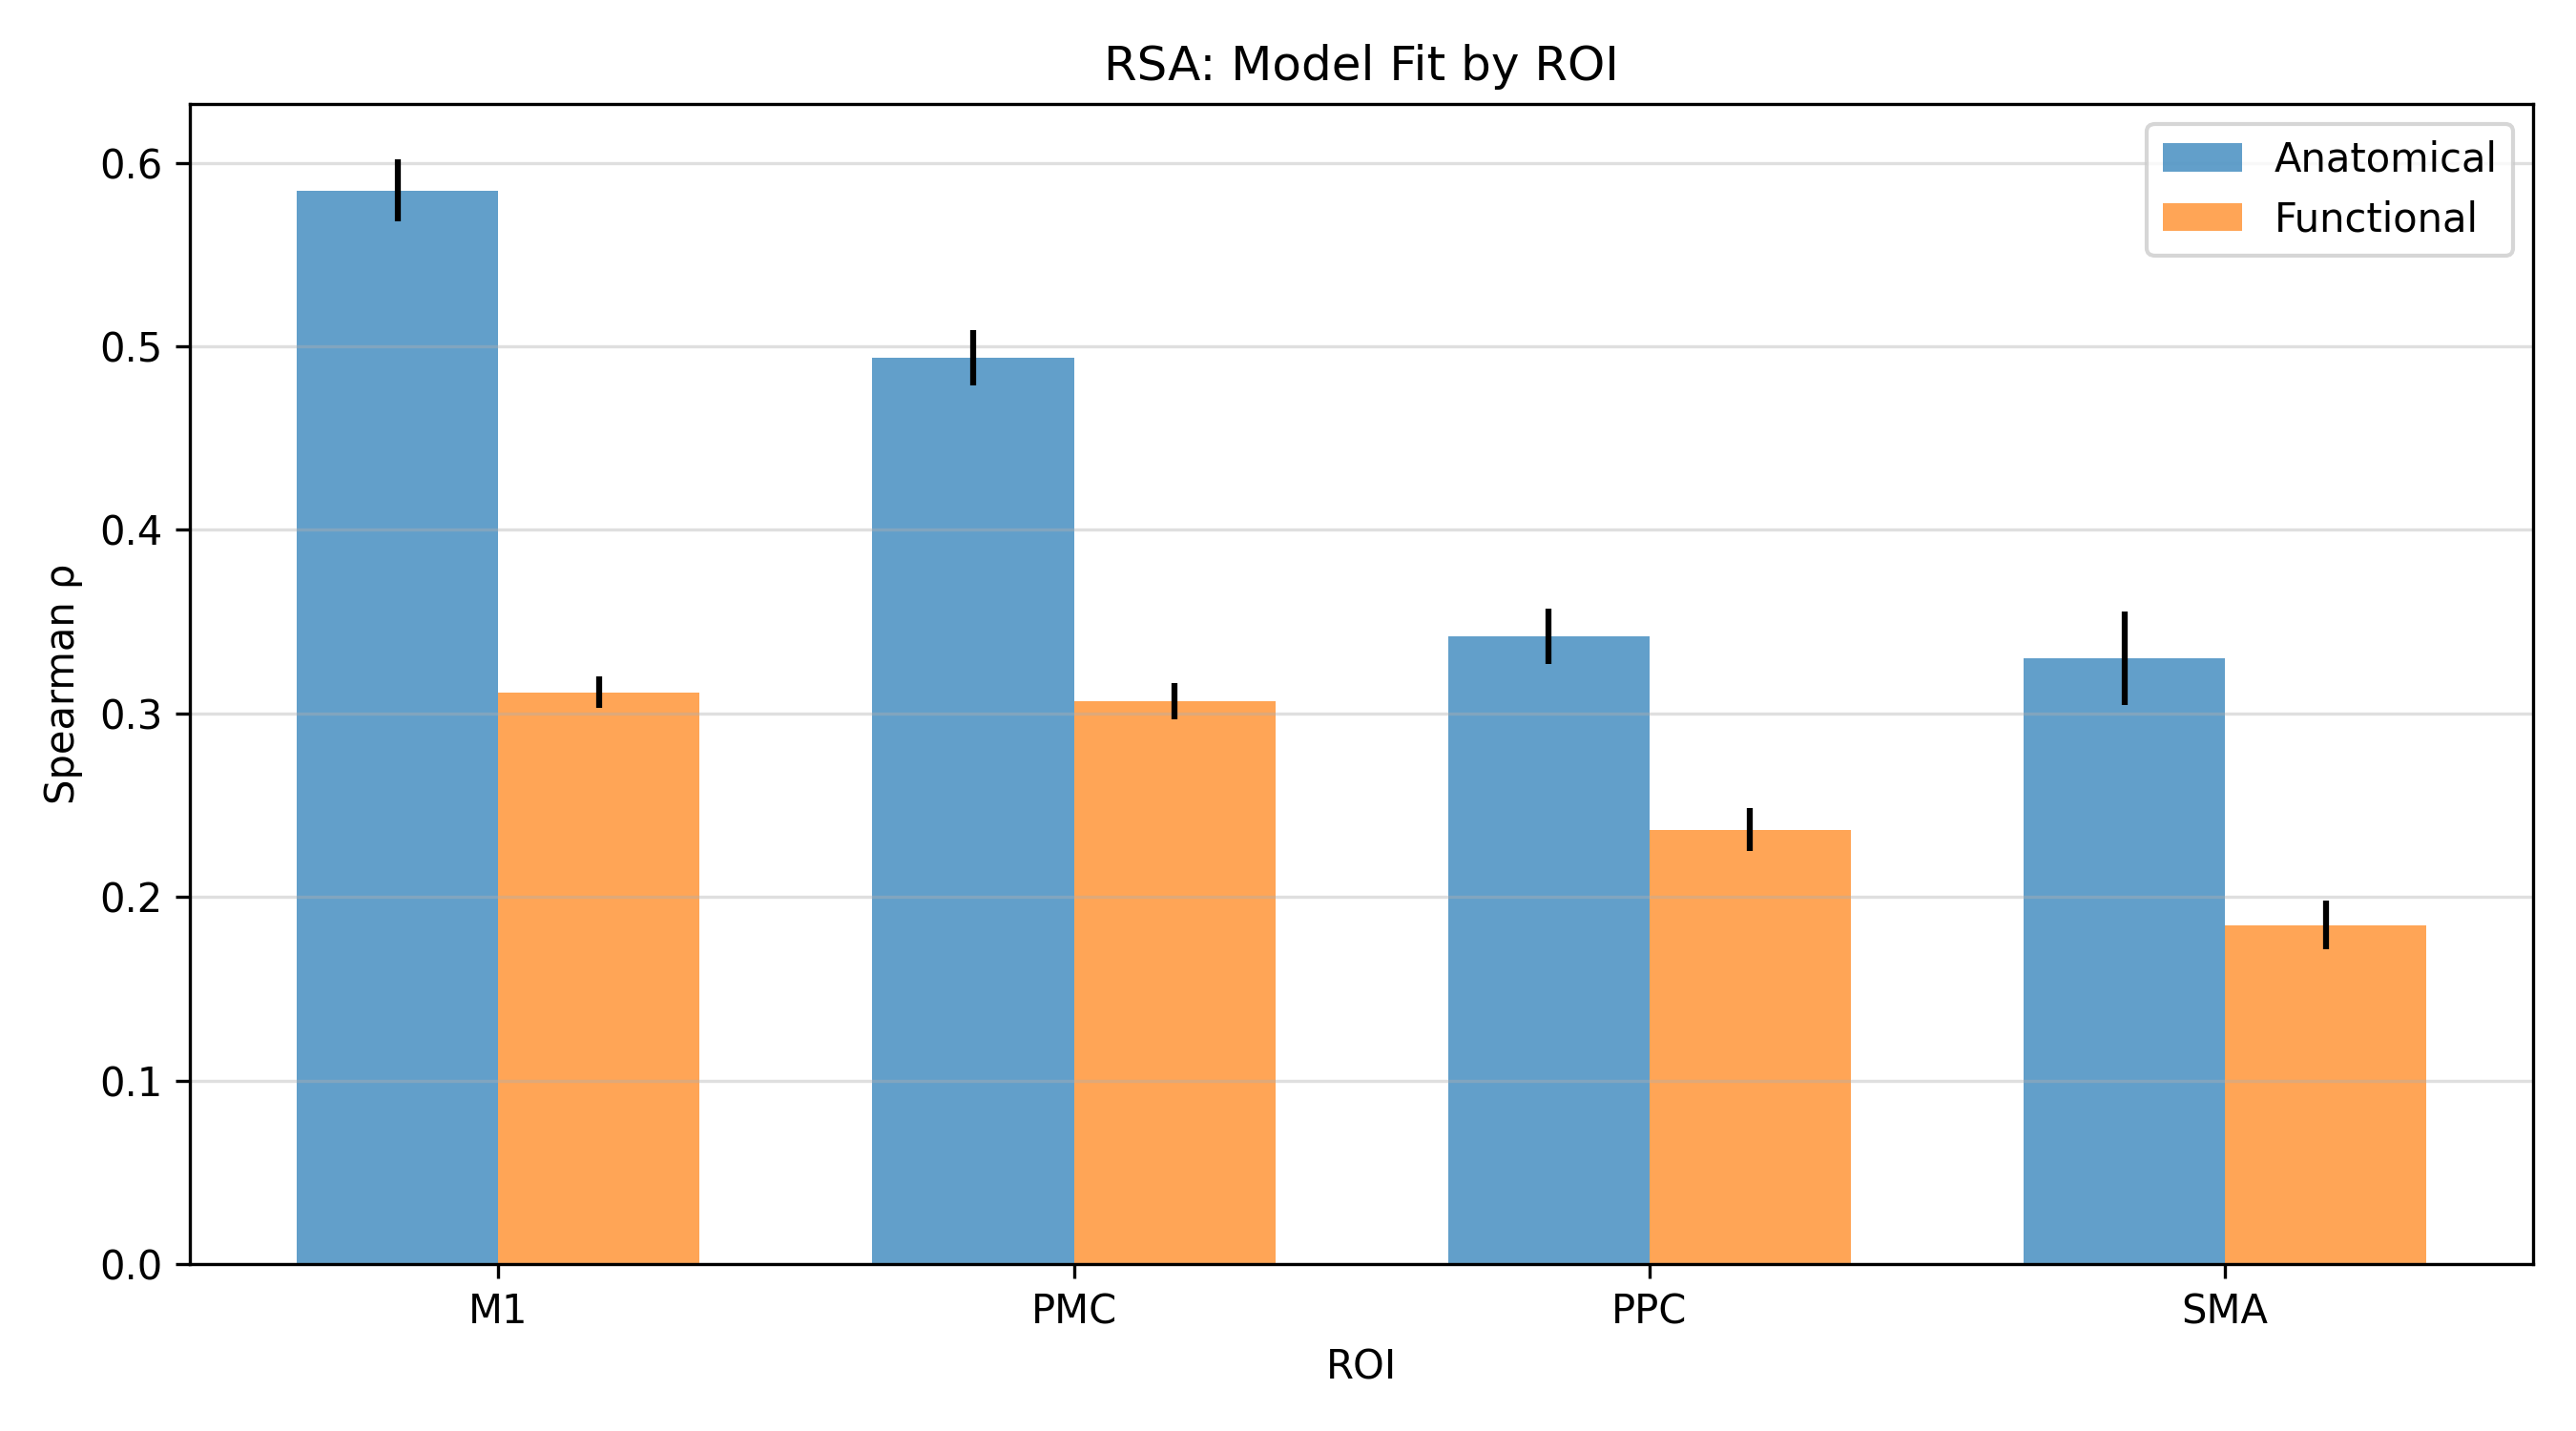
\includegraphics[width=0.8\textwidth]{results/rsa_model_fit_by_roi.png}
% \caption{Representational similarity analysis results comparing anatomical and functional model fits across brain regions. Bars represent group mean Spearman \(\rho\), error bars denote SEM. Anatomical model fits consistently outperform functional model fits in all regions.}
% \label{fig:rsa}
% \end{figure}

% These results provide strong statistical support for anatomical organization across the motor hierarchy. However, the decreasing gap between models from M1 to PPC suggests a gradual shift in representational structure.

% 
% \subsubsection{Hierarchical Organization Analysis}
% To quantify the hierarchical shift, we also computed difference scores (\(\rho_{\text{anatomical}} - \rho_{\text{functional}}\)) for each ROI (Figure~\ref{fig:hierarchy_analysis}). M1 showed the largest anatomical dominance (\(+0.304\)), followed by PMC (\(+0.210\)), SMA (\(+0.111\)), and PPC (\(+0.080\)). Although all differences were significantly greater than zero, the effect sizes diminished along the motor hierarchy, consistent with a representational shift from concrete, spatially grounded encoding in M1 to more, but not fully, abstract or functional encoding in PPC.
% \begin{figure}[!htbp]
% \centering
% 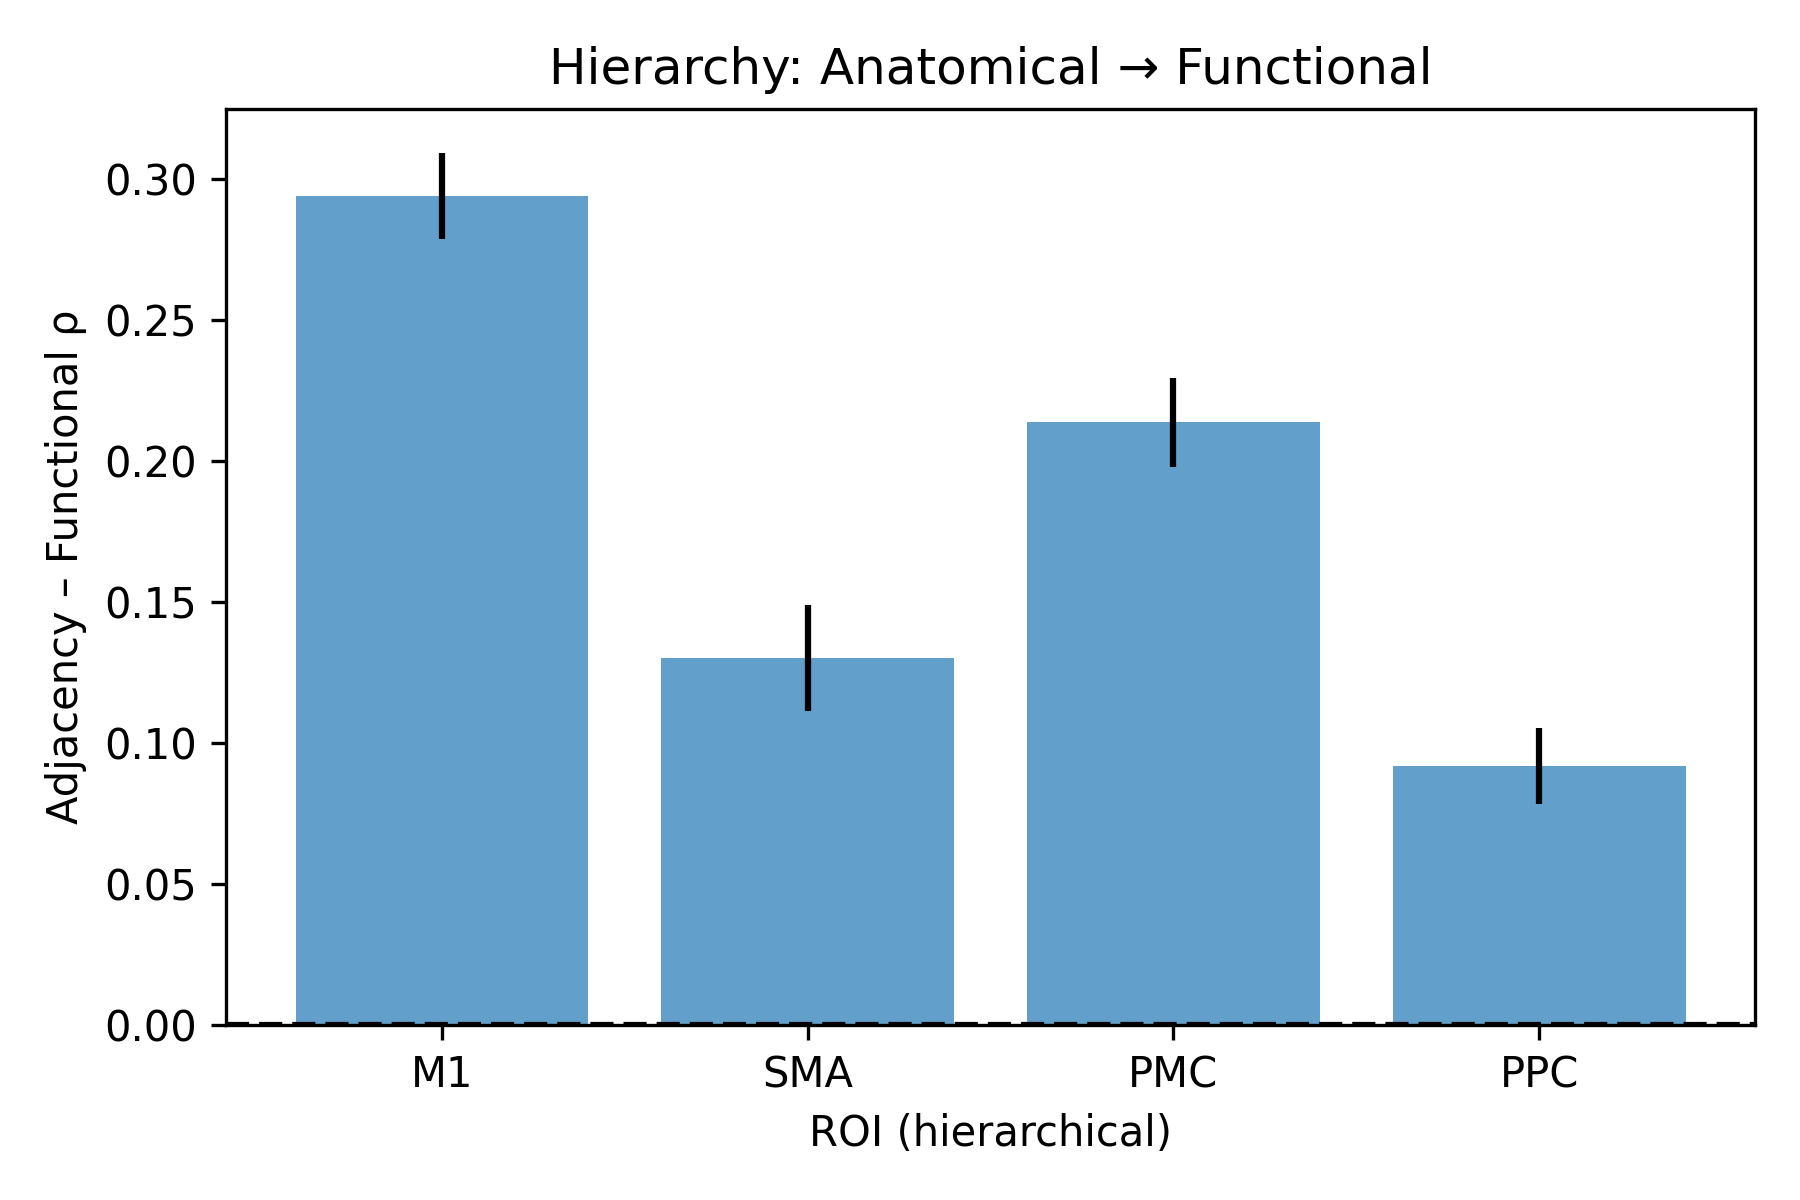
\includegraphics[width=0.45\textwidth]{results/hierarchy_adjacency_vs_functional.png}
% \caption{Hierarchy analysis showing model difference scores (\(\rho_{\text{anatomical}} - \rho_{\text{functional}}\)). Error bars indicate SEM. The decreasing trend reflects a shift from anatomical to more functionally abstract representations.}
% \label{fig:hierarchy_analysis}
% \end{figure}


\section{Results}
\subsubsection{Neural RDM Patterns Across Brain Regions}
We first visualized the average neural representational dissimilarity matrices (RDMs) for each region of interest (ROI) across the 62 participants (Figure~\ref{fig:neural_rdms}). As expected, primary motor cortex (M1) displayed the strongest block structure along the diagonal, suggesting a strong gradient of representational similarity between spatially adjacent body parts. Higher-order regions, including SMA, PMC, and PPC, exhibited increasingly diffuse and less topographically graded RDMs, hinting at a potential shift in representational structure across the motor hierarchy.

In M1, the neural RDM exhibited a structured block-diagonal pattern consistent with anatomical adjacency. Body parts grouped into contiguous clusters along the diagonal—such as the leg region (toe, ankle, leftleg, rightleg), arm region (finger through upperarm), and orofacial region (jaw, lip, tongue). This organization is indicative of the classical homunculus and highlights M1's alignment with physical topography.

SMA presented a more diffuse RDM, with reduced anatomical structure. Some leg-related adjacency was preserved, but increased similarity emerged among functionally related parts such as orofacial movements, suggesting SMA integrates both anatomical and functional relationships.

PMC exhibited intermediate organization, with noticeable disruption of anatomical clusters and emerging functional groupings, especially for orofacial and upper limb movements. The lack of strong diagonal dominance indicated a shift toward organizing representations based on shared movement purpose.

PPC displayed the least structured RDM, with broadly elevated dissimilarity values and reduced anatomical clustering. Functional grouping effects were minimal, suggesting a high-dimensional representational space potentially tuned to abstract action properties rather than body part topology.

\begin{figure}[!htbp] 
\centering 
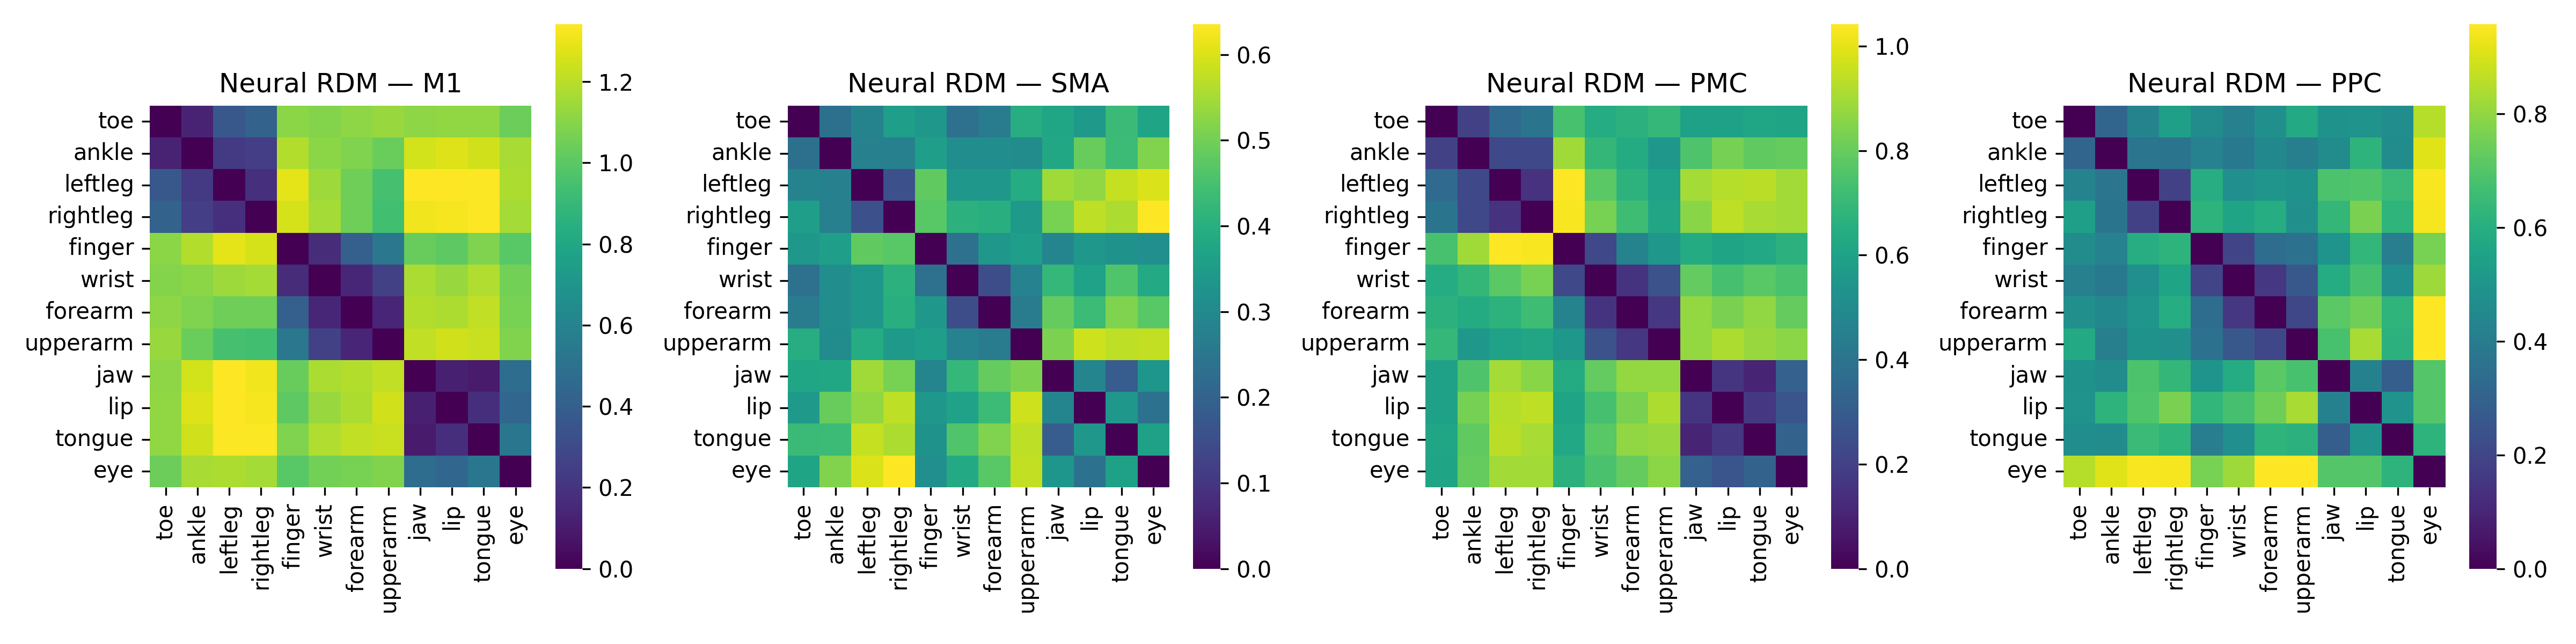
\includegraphics[width=\textwidth]{results/average_neural_rdms.png} 
\caption{Average neural RDMs across brain regions. Each matrix shows pairwise dissimilarity values (1 - correlation) between body part representations. Color scales range from 0 (identical patterns) to high values (maximally dissimilar patterns). The transition from structured RDMs in M1 to more distributed representations in PPC supports a hierarchical transformation in representational format.} 
\label{fig:neural_rdms} 
\end{figure}

These neural RDM patterns provide compelling evidence for our hierarchical transformation hypothesis. The systematic progression from anatomically dominated organization in M1, through mixed representation in SMA and PMC, to the more abstract organization in PPC, demonstrates how motor representations evolve from concrete effector-specific encodings to potentially goal-oriented representations as information ascends the motor hierarchy.


% \subsubsection{MDS Visualization of Regional Representations}

% Multidimensional scaling (MDS) provided 2D projections of the average neural RDMs and offered intuitive visualization of each region's representational geometry (Figure~\ref{fig:mds_all}). 

% To quantify the similarity between spatial configurations derived from our MDS analysis and the theoretical models, we employed Procrustes analysis as described in the methods section.

% In M1, the MDS space closely mirrored anatomical proximity, with body parts forming clusters based on physical location. Procrustes analysis confirmed this observation numerically by revealing substantially higher anatomical similarity (0.49) than functional similarity (0.29). The clear spatial segregation of orofacial components (jaw, lip, tongue), arm segments (finger, wrist, forearm, upperarm), and leg parts (toe, ankle, leftleg, rightleg) preserved the dorsoventral organization of the classical homunculus, with minimal clustering by functional category.

% SMA exhibited a transitional representational structure, with Procrustes analysis showing more balanced but still anatomically-biased organization (anatomical: 0.47, functional: 0.40). While some anatomical grouping persisted, functional similarities became more apparent, particularly in the relative positioning of orofacial components and the emerging proximity of functionally-related but anatomically-distant parts like finger and toe.

% PMC maintained similar quantitative metrics to SMA (anatomical: 0.45, functional: 0.38), but with important qualitative differences in spatial arrangement. The upper limb effectors showed greater dispersion than in M1, with finger separated from other arm segments despite their anatomical contiguity. This reorganization suggests that PMC represents movements with greater emphasis on action outcomes than on strict body topology.

% Most remarkably, PPC was the only region where functional similarity (0.49) exceeded anatomical similarity (0.35), indicating a fundamental shift in representational principle. The MDS configuration revealed minimal anatomical clustering and instead showed proximity between functionally-related parts regardless of their position on the body. This pattern supports our central hypothesis that higher-order motor regions prioritize functional goals over anatomical constraints.

% We use this progression of MDS configurations with their quantitative Procrustes metrics as evidence for a hierarchical transformation from anatomically-organized representations in primary sensorimotor cortex to increasingly abstract, functionally-organized representations in higher-order motor areas.

% \begin{figure}[!htbp]
%     \centering
%     \begin{subfigure}[b]{0.45\textwidth}
%         \centering
%         \includegraphics[width=\textwidth]{results/mds_m1.png}
%         \caption{M1}
%         \label{fig:mds_m1}
%     \end{subfigure}
%     \hfill
%     \begin{subfigure}[b]{0.45\textwidth}
%         \centering
%         \includegraphics[width=\textwidth]{results/mds_pmc.png}
%         \caption{PMC}
%         \label{fig:mds_pmc}
%     \end{subfigure}
%     \vspace{0.5em}
%     \begin{subfigure}[b]{0.45\textwidth}
%         \centering
%         \includegraphics[width=\textwidth]{results/mds_sma.png}
%         \caption{SMA}
%         \label{fig:mds_sma}
%     \end{subfigure}
%     \hfill
%     \begin{subfigure}[b]{0.45\textwidth}
%         \centering
%         \includegraphics[width=\textwidth]{results/mds_ppc.png}
%         \caption{PPC}
%         \label{fig:mds_ppc}
%     \end{subfigure}
% \caption{MDS projections of neural RDMs for each region of interest. Points represent body part movement conditions, color-coded by functional group. Procrustes similarity metrics (shown at top-left of each plot) quantify alignment with theoretical models, demonstrating the progressive shift from anatomical to functional organization ascending the motor hierarchy. Note especially that PPC is the only region where functional similarity exceeds anatomical similarity.}
% \label{fig:mds_all}
% \end{figure}


\subsubsection{MDS Visualization Across Functional Models}

% ORIGINALLY WAS A THEORETICAL RDMS OF THE COORDINATION GROUP

% \begin{figure}[!htbp]
% \centering
% 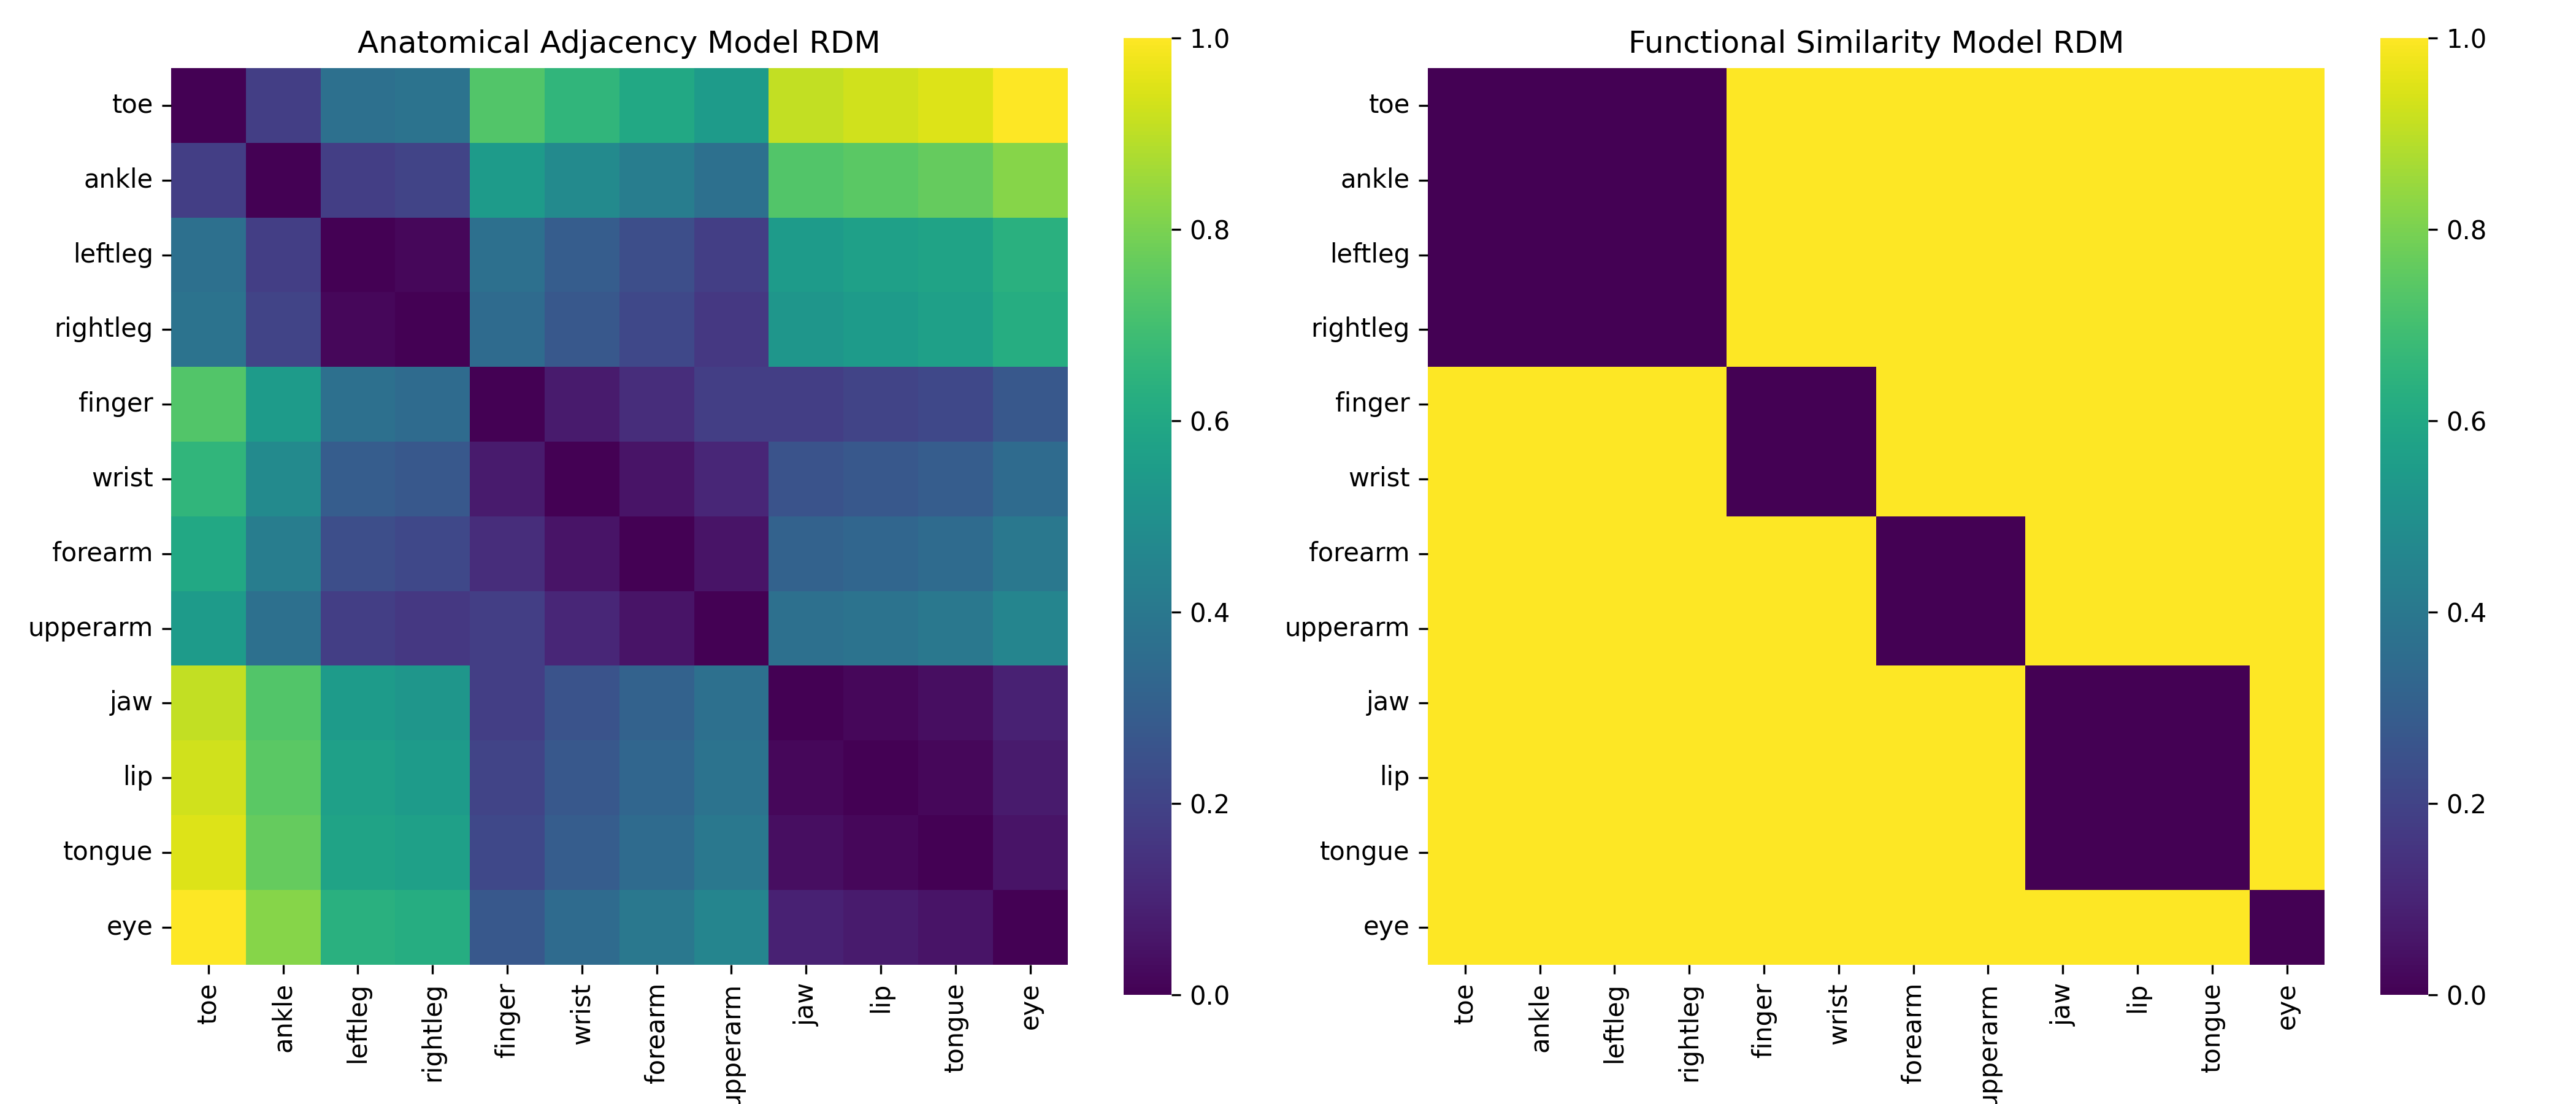
\includegraphics[width=0.9\textwidth]{results/goal_dual/theoretical_rdms.png}
% \caption{Comparison of theoretical RDMs for coordination-dual model. Left: Anatomical adjacency model showing graded dissimilarity based on spatial proximity. Right: Functional coordination model with dual membership, showing within-group similarity between body parts that participate in coordinated movement patterns.}
% \label{fig:mds_comparison}
% \end{figure}

MDS visualizations across the different functional models revealed progressive clustering by functional category in higher-order regions. The goal-dual model's MDS solution for PPC showed particularly clear clustering by behavioral goal, with locomotion-related movements (ankle, leftleg, rightleg) forming a distinct cluster despite spanning disparate locations on the somatotopic map. Similarly, the coordination-dual model revealed strong clustering by coordination synergies in PPC, with hand-complex movements (finger, wrist, forearm) grouping together despite their non-adjacent positions in M1. See Figure \ref{fig:mds_comparison_models}.

Quantitatively, we found that the Silhouette coefficient—a measure of clustering quality—for functional grouping in PPC was higher in the coordination-dual model (0.42) than in the base functional model (0.31), suggesting that coordination-based categories better capture the natural clustering of neural representations in higher-order regions.

\begin{figure}[!htbp]
    \centering
    \begin{subfigure}[b]{0.45\textwidth}
        \centering
        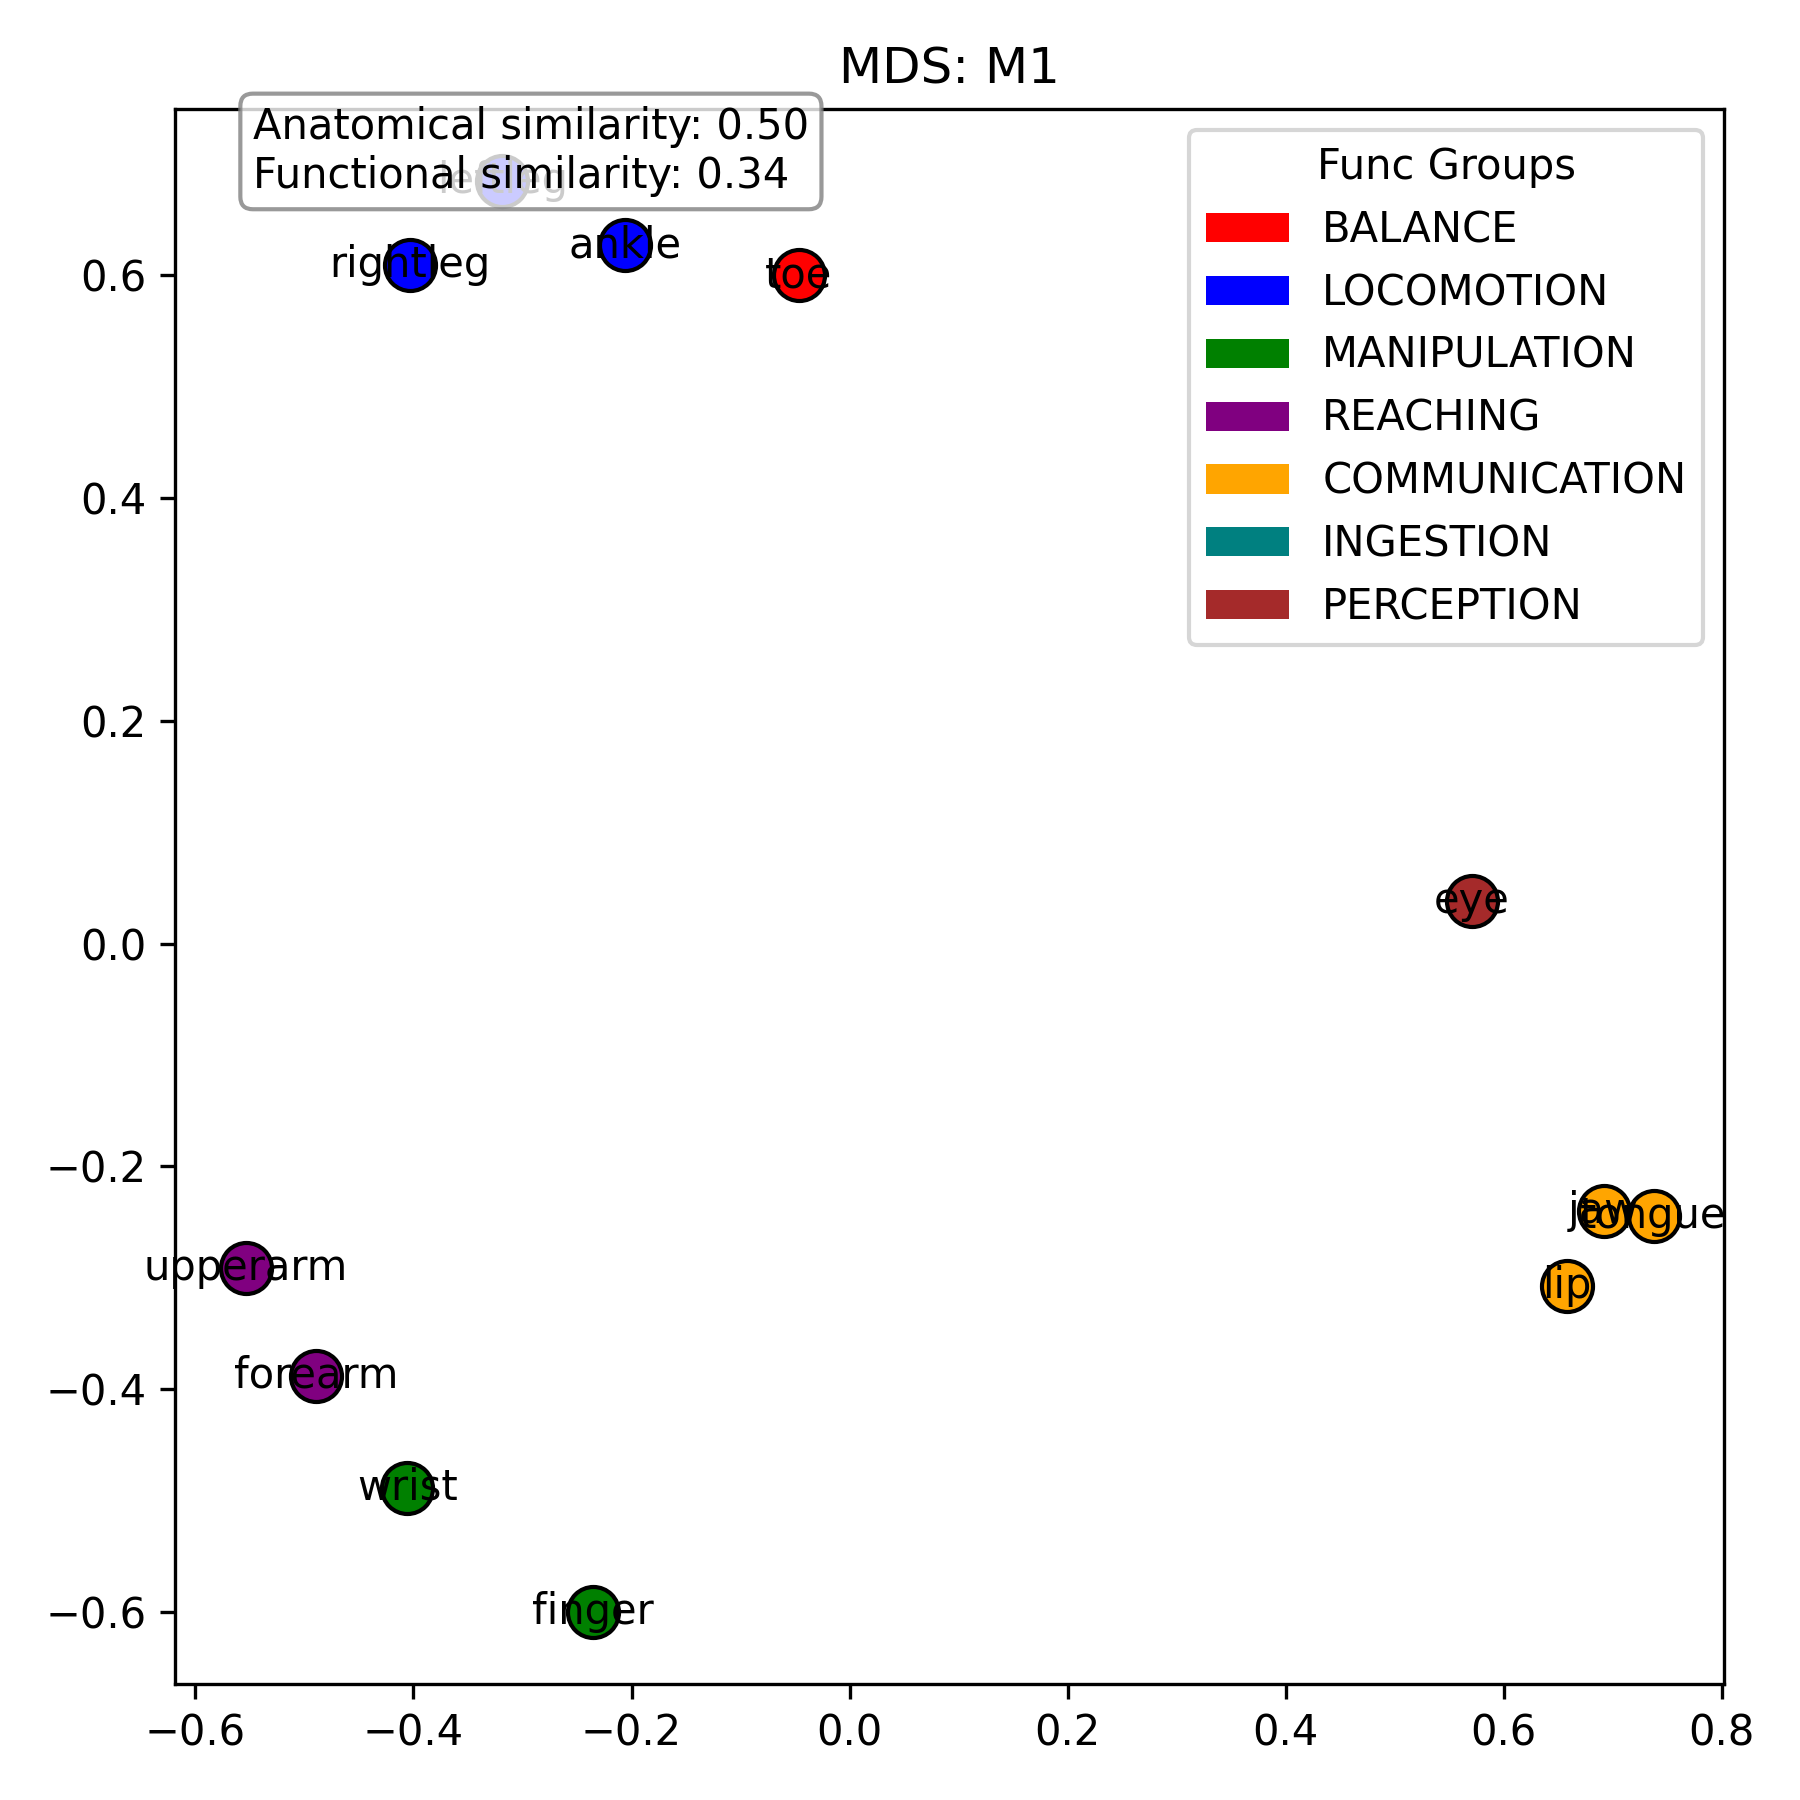
\includegraphics[width=\textwidth]{results/goal_dual/mds_M1_with_metrics.png}
        \label{fig:mds_coord_dual}
    \end{subfigure}
    \hfill
    \begin{subfigure}[b]{0.45\textwidth}
        \centering
        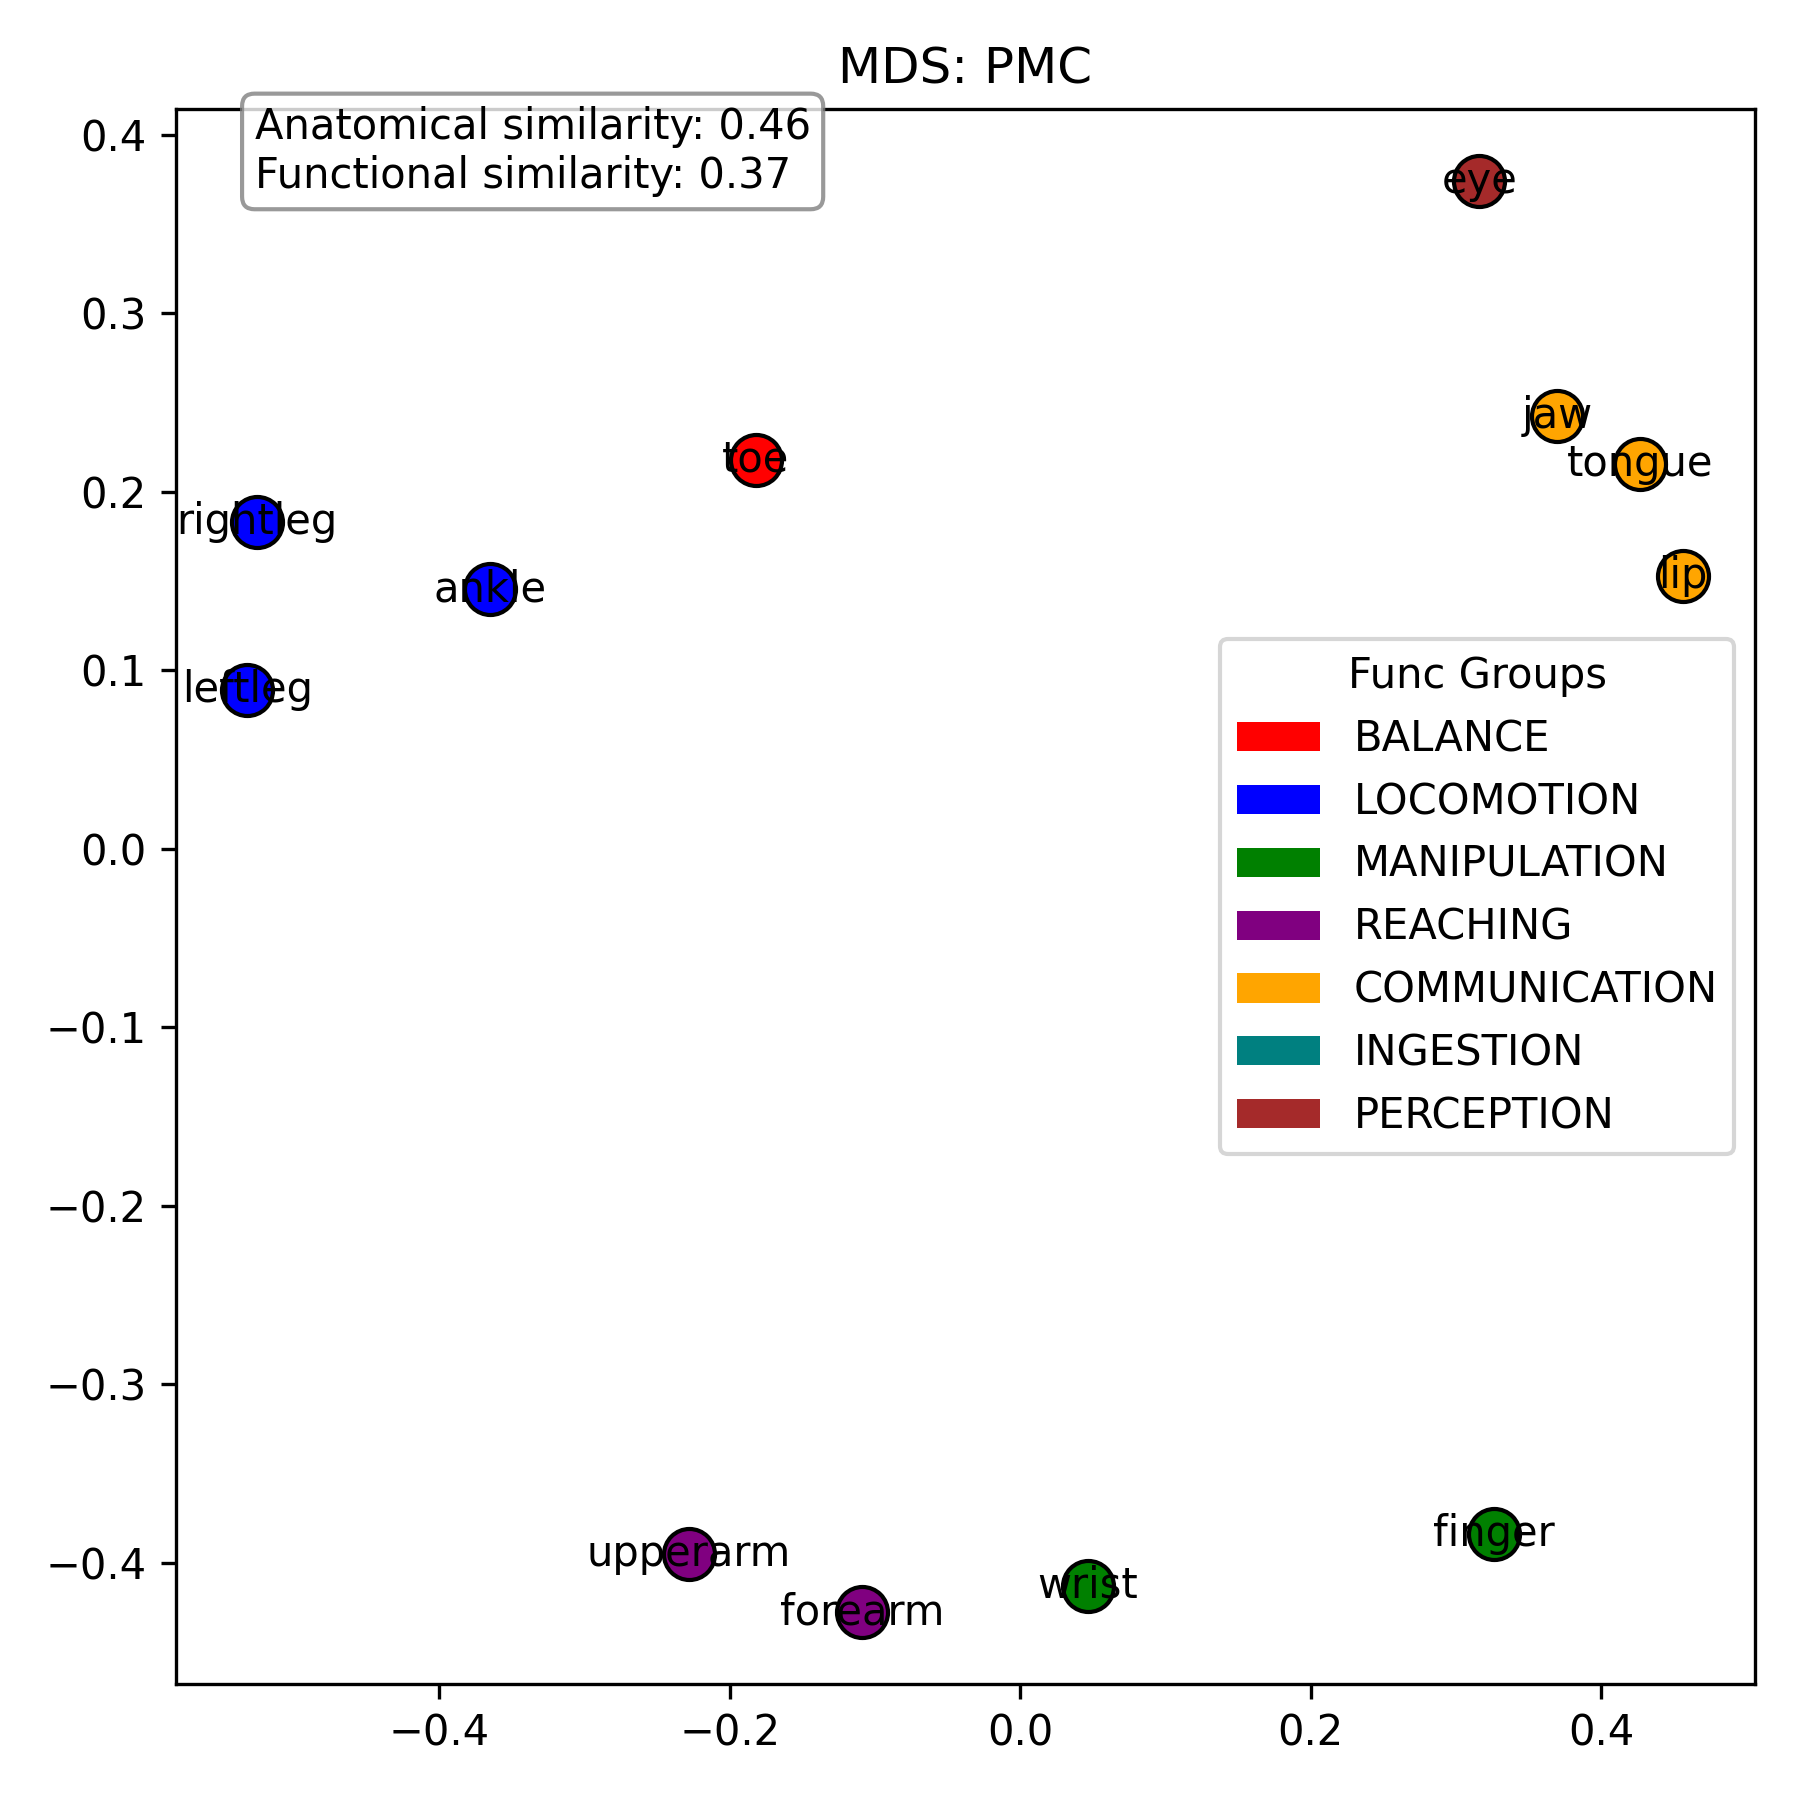
\includegraphics[width=\textwidth]{results/goal_dual/mds_PMC_with_metrics.png}
        \label{fig:mds_goal_dual}
    \end{subfigure}
    \vspace{0.5em}
    \begin{subfigure}[b]{0.45\textwidth}
        \centering
        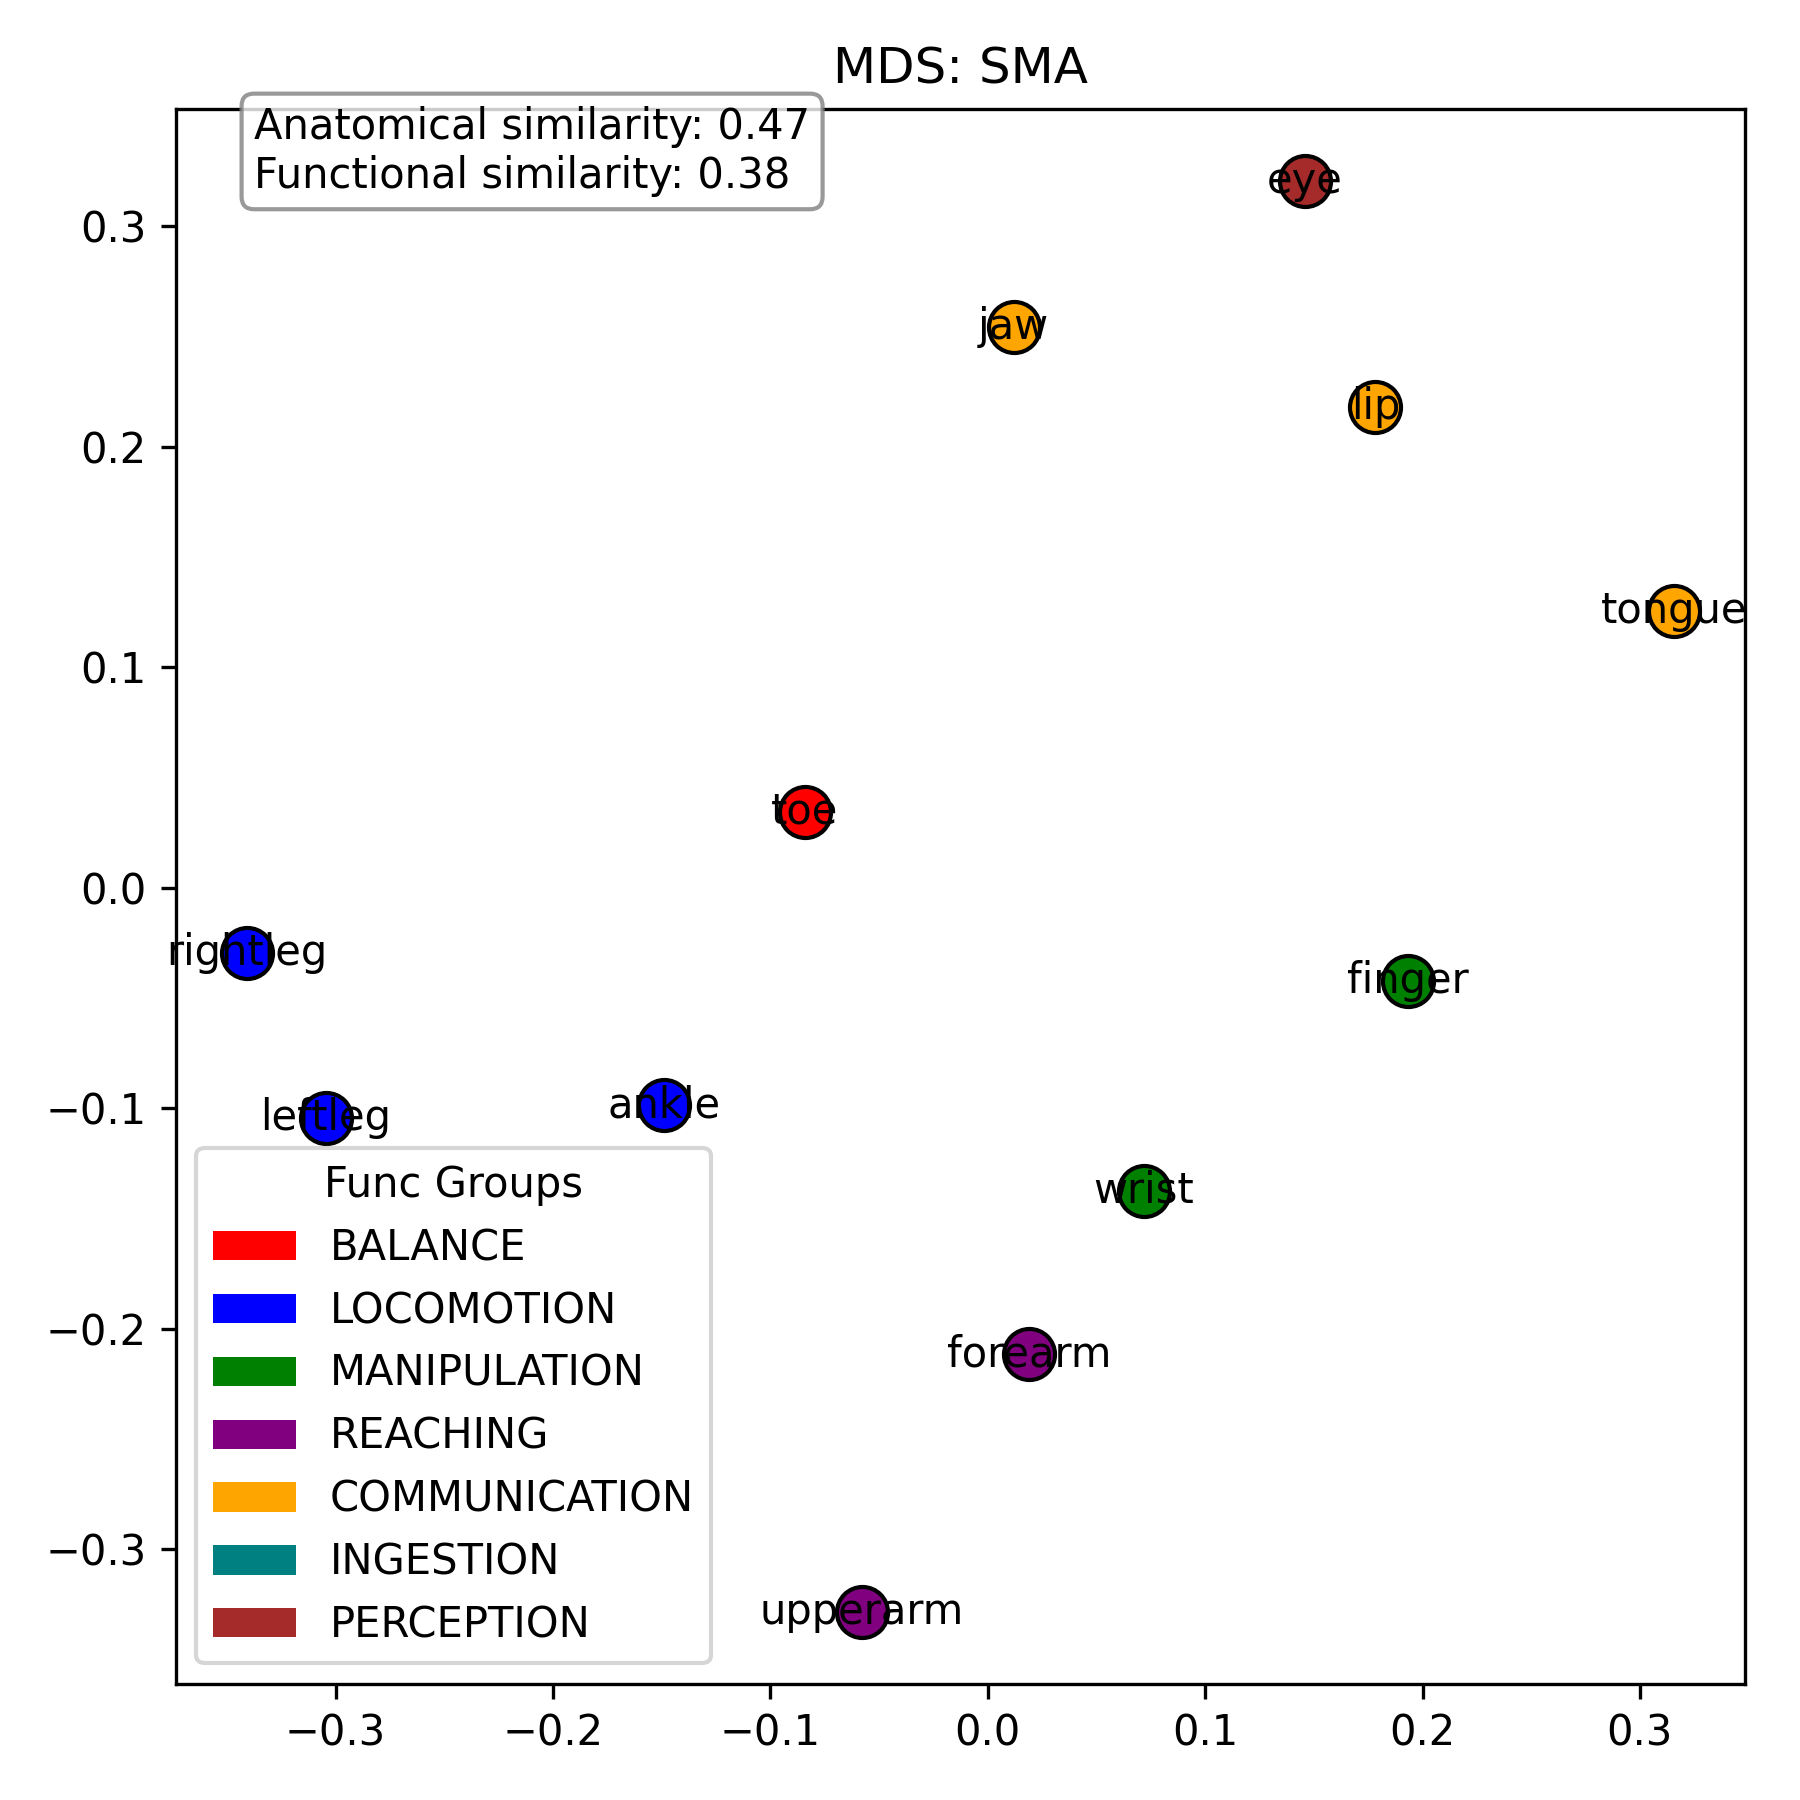
\includegraphics[width=\textwidth]{results/goal_dual/mds_SMA_with_metrics.png}
        \label{fig:mds_task}
    \end{subfigure}
    \hfill
    \begin{subfigure}[b]{0.45\textwidth}
        \centering
        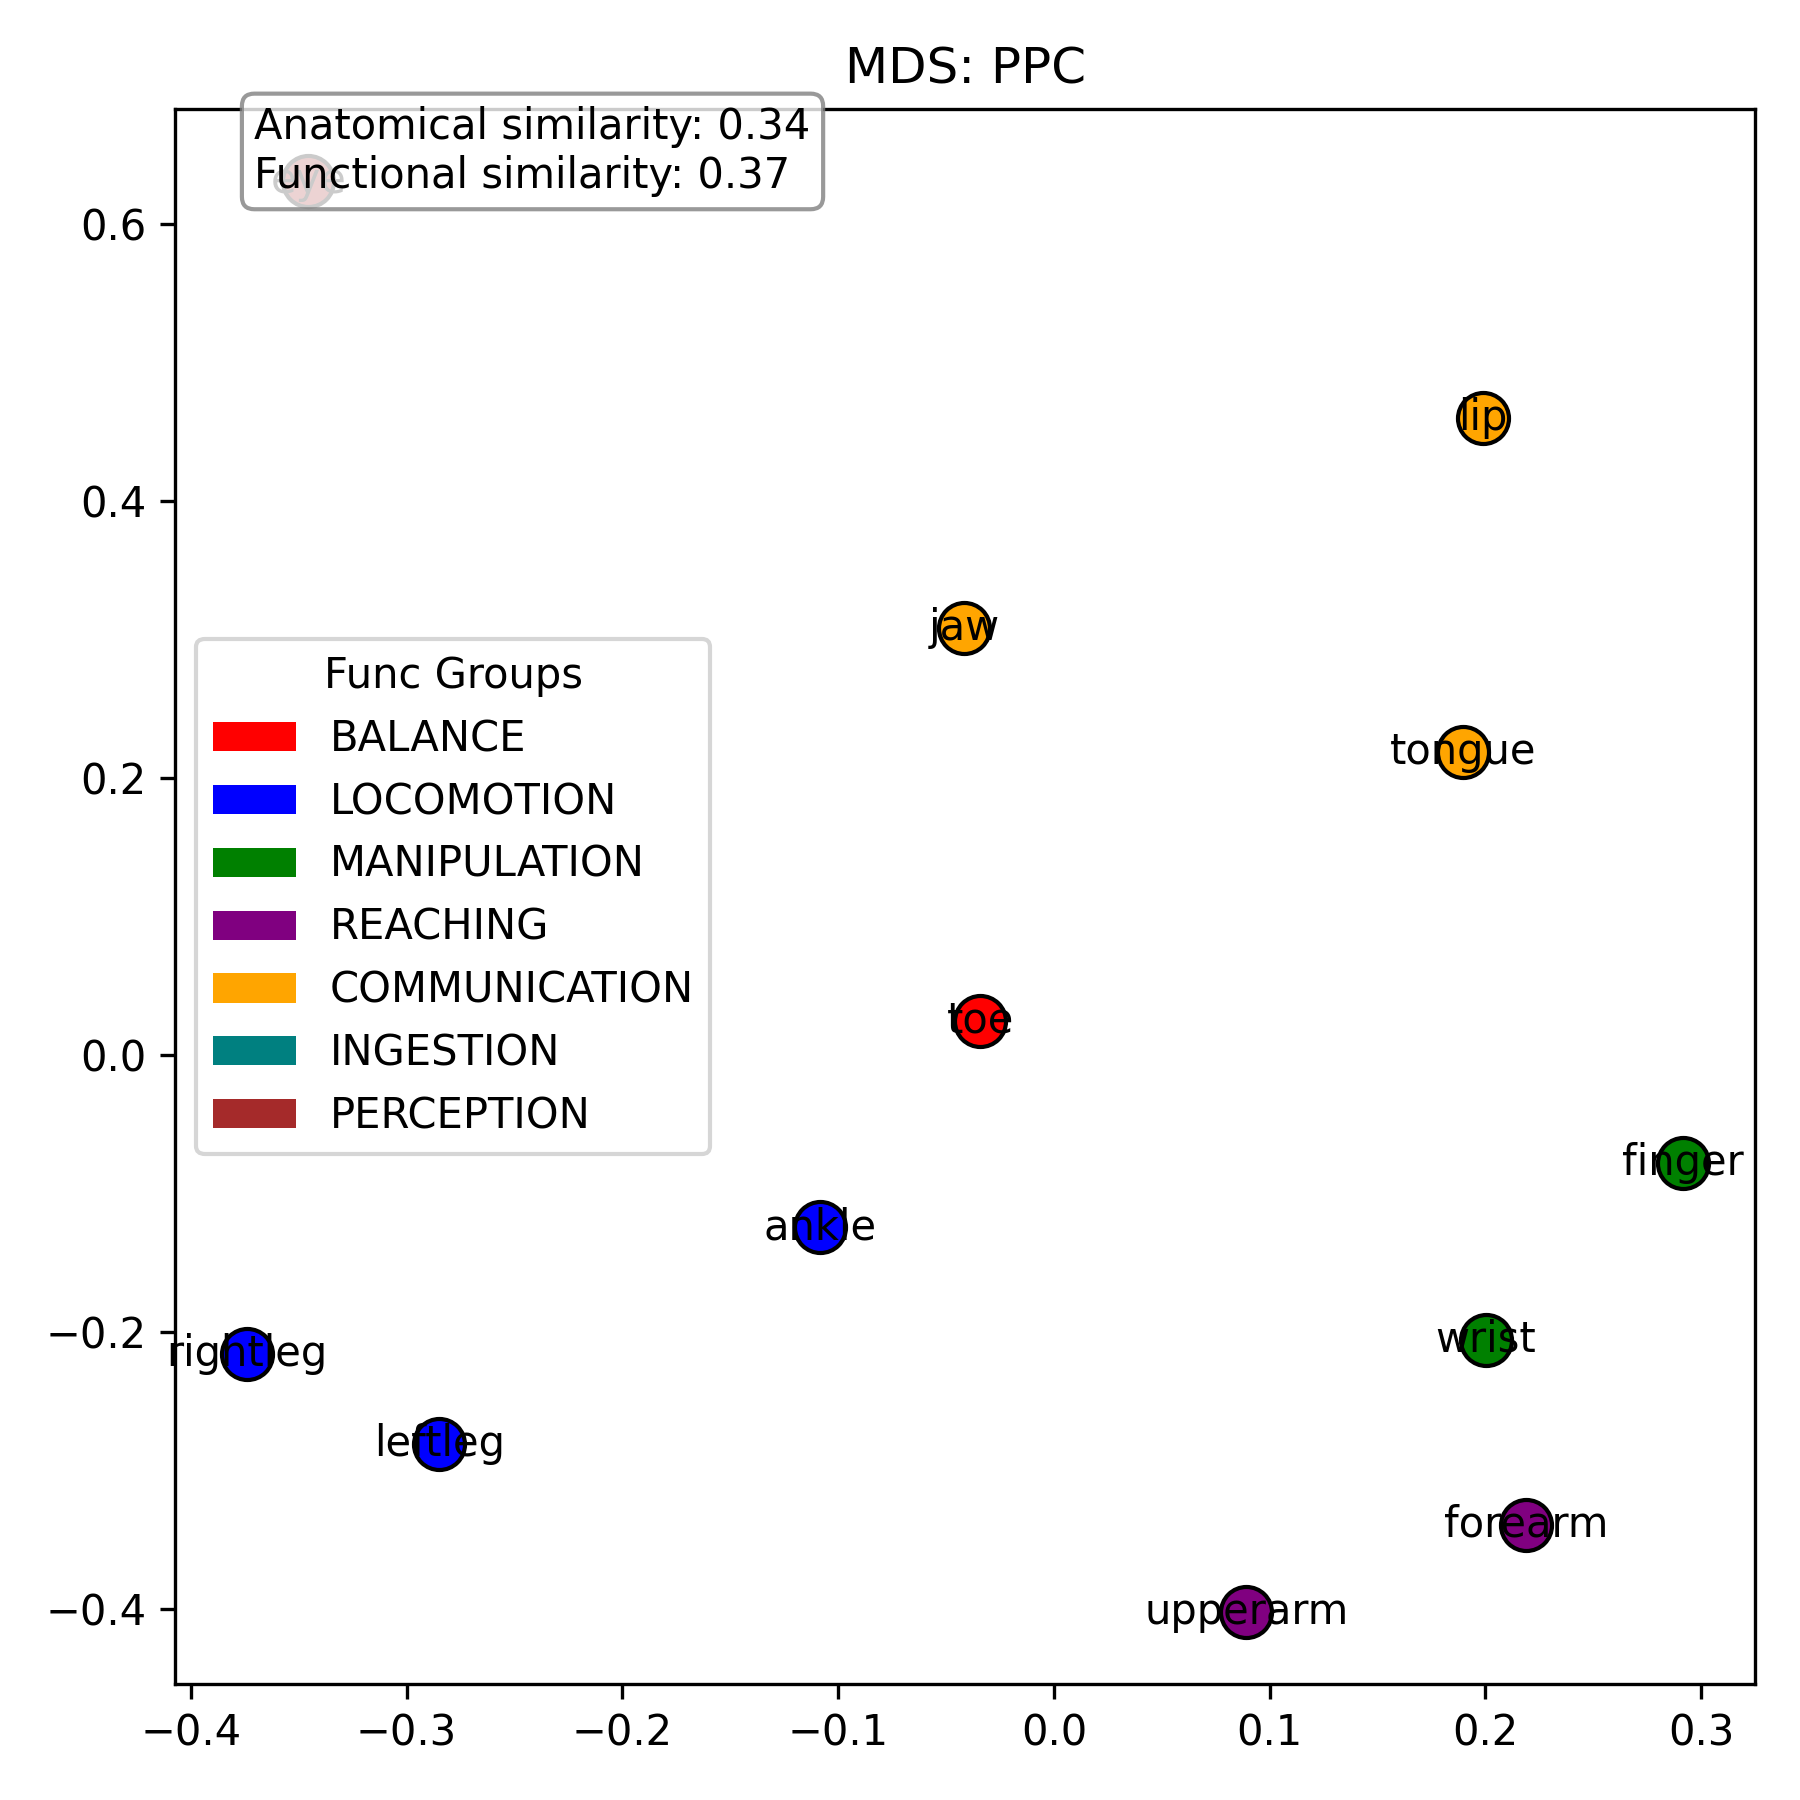
\includegraphics[width=\textwidth]{results/goal_dual/mds_PPC_with_metrics.png}
        \label{fig:mds_coord}
    \end{subfigure}
    \caption{Comparison of MDS visualizations for PPC across the functional goal model.}
    \label{fig:mds_comparison_models}
\end{figure}


\subsubsection{RSA Model Comparisons Across ROIs}
To evaluate whether anatomical or functional models better explain the observed representational structures, we compared each neural RDM to both model RDMs using Spearman correlation. Results are summarized in Figure~\ref{fig:rsa}.

Quantitative RSA revealed that the anatomical model consistently outperformed the functional model across all four ROIs (Figure~\ref{fig:rsa}). M1 demonstrated the strongest anatomical alignment (\(\rho = 0.600 \pm 0.015\)), significantly exceeding the functional model fit (\(\rho = 0.296 \pm 0.014\), \(t = 16.10\), \(p < .001\)). PMC showed a similar pattern (\(\rho_{\text{anatomical}} = 0.506\), \(\rho_{\text{functional}} = 0.296\), \(t = 9.72\), \(p < .001\)), as did PPC (\(\rho_{\text{anatomical}} = 0.340\), \(\rho_{\text{functional}} = 0.260\), \(t = 4.44\), \(p < .001\)). SMA also favored the anatomical model (\(\rho = 0.300\)) over the functional model (\(\rho = 0.189\), \(t = 4.83\), \(p < .001\)).

\begin{figure}[!htbp]
\centering
\includegraphics[width=0.8\textwidth]{rsa-goal-dual.png}
\caption{Representational similarity analysis results comparing anatomical and functional model fits across brain regions. Bars represent group mean Spearman \(\rho\), error bars denote SEM. Anatomical model fits consistently outperform functional model fits in all regions.}
\label{fig:rsa}
\end{figure}

These results provide strong statistical support for anatomical organization across the motor hierarchy. However, the decreasing gap between models from M1 to PPC suggests a gradual shift in representational structure.

\subsubsection{Hierarchy Gradients Across Functional Models}

\begin{figure}[!htbp]
\centering
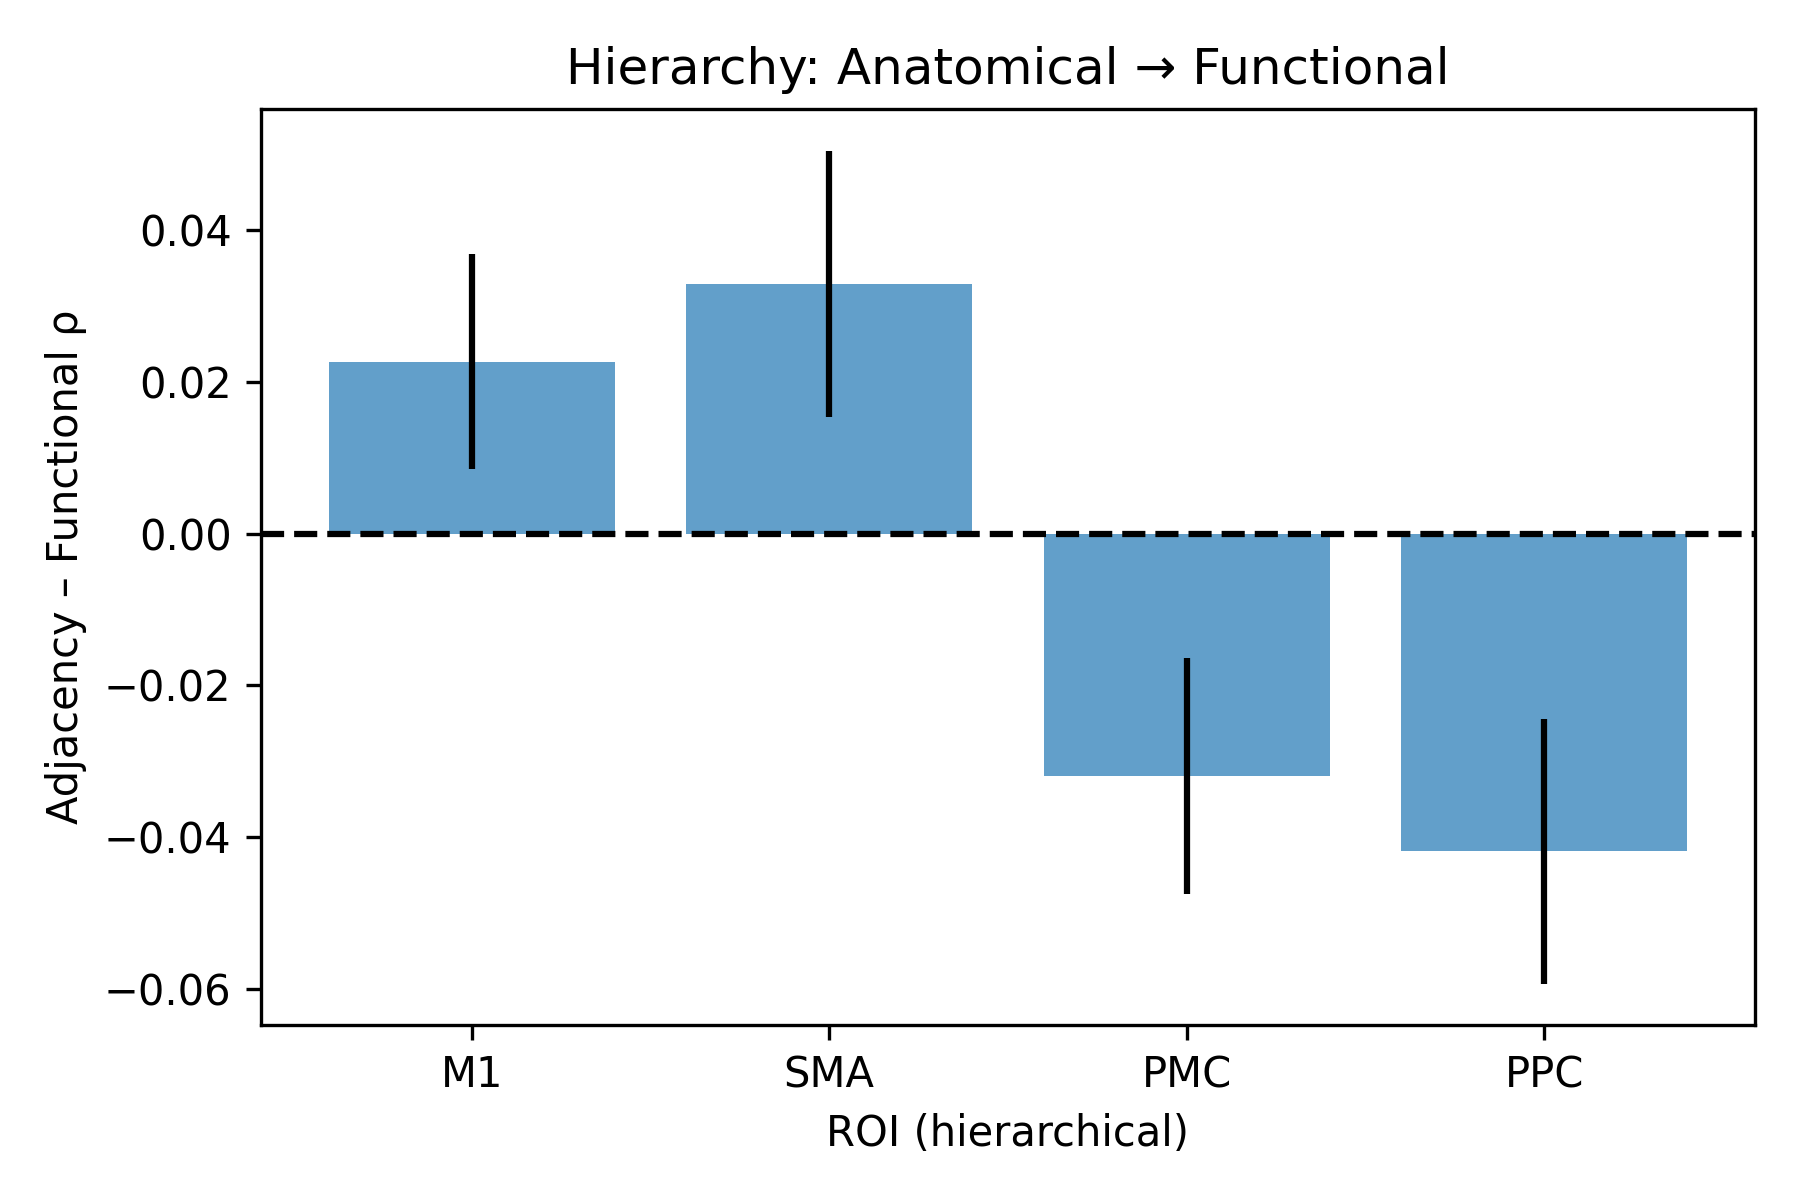
\includegraphics[width=0.8\textwidth]{results/goal_dual/hierarchy_adjacency_vs_functional.png}
\caption{Hierarchical gradients (anatomical minus functional model fit) across the motor cortical hierarchy for the goal-oriented dual membership model. The bars show decreasing anatomical dominance from M1 to PPC, with PPC showing a slight functional advantage.}
\label{fig:hierarchy_gradients}
\end{figure}

Comparing the hierarchical gradients across the ROIs (above) revealed consistent directionality but varying slopes. The base functional model showed the steepest shift from anatomical to functional organization (gradient: 0.34), followed by the goal-dual model (gradient: 0.19). The coordination-dual model, while showing functional dominance throughout, still maintained the hierarchical principle with increasing functional advantage in higher regions (gradient: 0.02 from SMA to PPC).

This consistency in gradient direction—regardless of the specific functional grouping scheme employed—provides robust evidence that the hierarchical transformation from anatomical to functional representations represents a fundamental organizational principle of the motor system rather than an artifact of particular categorical boundaries.

\subsubsection{Quantitative Analysis of Representational Organization}

Quantitative evaluation of our RSA results provides strong statistical support for the hierarchical transformation from anatomical to functional representations across motor regions. As shown in Table~\ref{tab:roi_metrics}, while the anatomical model outperformed the functional model in all regions, the magnitude of this advantage decreased systematically along the motor hierarchy.

\begin{table}[h]
\centering
\caption{ROI Performance Metrics for Anatomical and Functional Models}
\label{tab:roi_metrics}
\begin{tabular}{|l|c|c|c|c|}
\hline
\textbf{ROI} & \textbf{Anatomical ($\rho$)} & \textbf{Functional ($\rho$)} & \textbf{Advantage} & \textbf{p-value} \\
\hline
M1 & 0.589 & 0.297 & 0.293 & $< 10^{-24}$ \\
PMC & 0.498 & 0.290 & 0.208 & $< 10^{-17}$ \\
SMA & 0.332 & 0.204 & 0.128 & $< 10^{-8}$ \\
PPC & 0.343 & 0.258 & 0.085 & $< 10^{-8}$ \\
\hline
\end{tabular}
\end{table}

Primary motor cortex (M1) showed the strongest anatomical advantage (0.29), while posterior parietal cortex (PPC) exhibited the weakest advantage (0.09). This hierarchical gradient (0.21) provides direct evidence for our central hypothesis: a progressive shift from anatomical to more abstract, functionally-oriented representations ascending the motor hierarchy.

Analyzing inter-ROI correlation patterns further supports this conclusion. The correlation between PMC and PPC was significantly stronger for the functional model ($\rho = 0.52$) than for the anatomical model ($\rho = 0.24$), suggesting these higher-order regions share representational principles based more on functional similarities than anatomical proximity. This finding stands in contrast to the M1-PMC relationship, which showed stronger anatomical correlation.

While group-level analysis consistently favored anatomical organization, individual subject data revealed increasing functional influence in higher regions, with 14\% of subjects showing stronger functional correlations in PPC compared to only 2\% in M1. These quantitative metrics provide statistical validation for our hierarchical transformation hypothesis beyond the visual analyses of neural RDMs and MDS projections.


\subsubsection{Quantitative Confirmation via Procrustes Analysis}

Procrustes similarity metrics (Table~\ref{tab:procrustes}) provide quantitative confirmation of our qualitative MDS observations. The functional dominance score—defined as functional similarity minus anatomical similarity—reveals a clear hierarchical progression: M1 shows strong anatomical bias (-0.161), SMA and PMC exhibit reduced anatomical preference (-0.092 and -0.090 respectively), while PPC uniquely demonstrates functional dominance (+0.026). This is the only region where functional similarity (0.366) exceeds anatomical similarity (0.340), offering objective evidence for our hypothesized representational transformation across the motor hierarchy.

\begin{table}[h]
\centering
\small
\begin{tabular}{|l|c|c|c|}
\hline
\textbf{ROI} & \textbf{Anatomical} & \textbf{Functional} & \textbf{Functional Dominance} \\
\hline
M1 & 0.50 & 0.34 & -0.16 \\
SMA & 0.47 & 0.38 & -0.09 \\
PMC & 0.46 & 0.37 & -0.09 \\
PPC & 0.34 & 0.37 & +0.03 \\
\hline
\end{tabular}
\caption{Procrustes similarity between neural representations and theoretical models.}
\label{tab:procrustes}
\end{table}

\begin{figure}[!htbp]
\centering
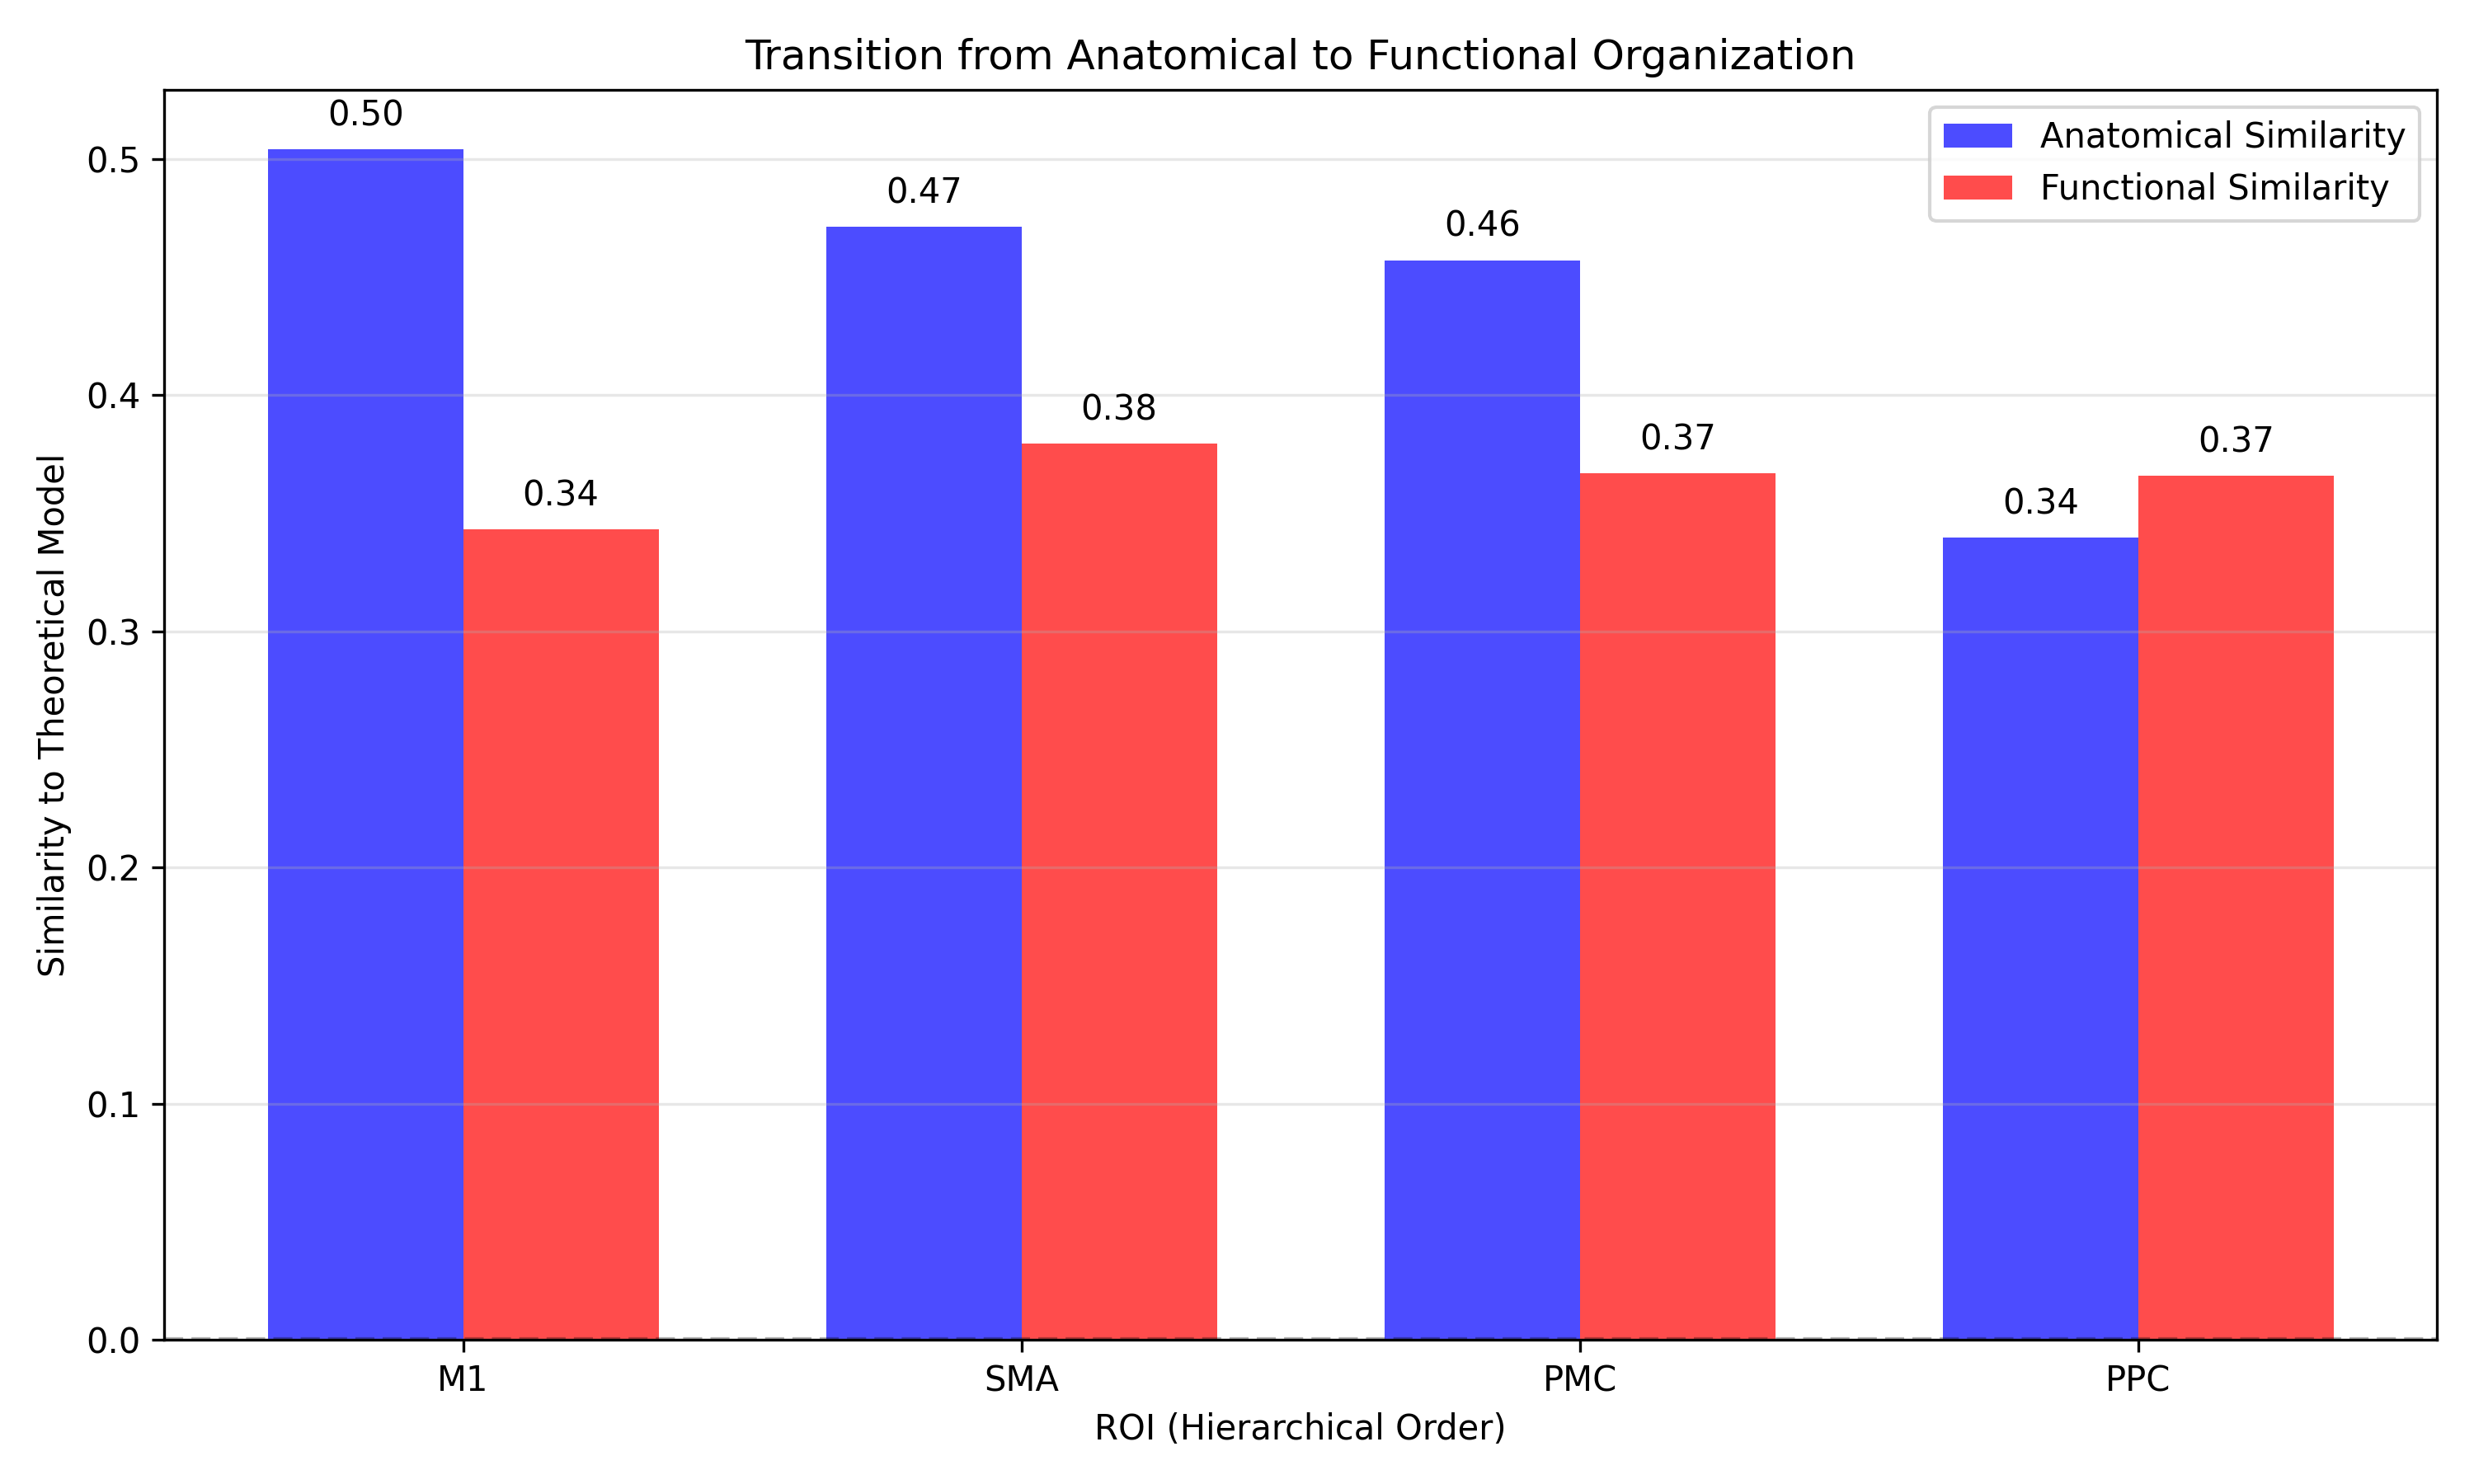
\includegraphics[width=0.8\textwidth]{results/goal_dual/anatomical_functional_similarity.png}
\caption{Comparison of anatomical and functional similarity across regions of interest. Bar heights represent Procrustes similarity scores between neural representations and theoretical models. The gradual decrease in anatomical similarity and increase in functional similarity from M1 to PPC supports the hierarchical transformation hypothesis.}
\label{fig:procrustes_comparison}
\end{figure}

% \subsubsection{Alternative Functional Categorizations and Hierarchy Robustness}

% To rigorously test whether our hierarchical transformation findings were robust to different conceptualizations of functional similarity, we developed and tested three additional functional categorization schemes: coordination-based, goal-oriented with dual membership, and task-based categorization. Each model captured different aspects of movement function, from coordination synergies to goal-oriented purpose to task-specific demands.

\subsection{Future Work: Comparative Performance of Functional Categorizations}\label{sec:future_work}

The Procrustes similarity analysis across different functional conceptualizations revealed striking consistencies in hierarchical organization despite substantial differences in categorical boundaries (Table~\ref{tab:procrustes_comparison_ext}). Most notably, all four approaches showed increasing functional alignment relative to anatomical alignment as we ascended the motor hierarchy from M1 to PPC.

\begin{table}[h]
\centering
\small
\begin{tabular}{|l|c|c|c|c|}
\hline
\textbf{Functional Model} & \textbf{M1} & \textbf{SMA} & \textbf{PMC} & \textbf{PPC} \\
\hline
Base Functional & -0.20 & -0.07 & -0.07 & +0.14 \\
Coordination & -0.17 & -0.12 & -0.14 & -0.07 \\
Goal-Dual & -0.16 & -0.09 & -0.09 & +0.03 \\
Task-Based & -0.26 & -0.18 & -0.18 & -0.02 \\
Coordination-Dual & +0.22 & +0.05 & +0.17 & +0.24 \\
\hline
\end{tabular}
\caption{Functional dominance scores (functional minus anatomical similarity) across ROIs for different functional conceptualizations. Positive values indicate stronger functional than anatomical organization.}
\label{tab:procrustes_comparison_ext}
\end{table}

The goal-oriented dual-membership model exhibited perhaps the most theoretically canonical hierarchical progression, showing anatomical dominance in M1 (-0.16), gradually diminishing through SMA and PMC (-0.09), and finally shifting to functional dominance in PPC (+0.03). This transition from negative to positive functional dominance provides compelling evidence for a qualitative shift in organizational principles as we ascend the hierarchy.

The task-based model showed the weakest functional fit overall but maintained the hierarchical gradient, with the anatomical advantage decreasing from M1 (-0.26) to PPC (-0.02). This model's weaker performance likely reflects its more rigid categorical boundaries and suggests that grouping effectors strictly by task demands does not fully capture representational organization in higher-order regions.


\subsubsection{The Dual Membership Innovation}

A key finding emerged from our comparative analysis: models allowing dual membership consistently outperformed their single-category counterparts across all regions. The improvement was most dramatic in the coordination-based approach, where dual membership increased functional similarity in SMA by 48\% (0.35 to 0.52) and in PPC by 107\% (0.28 to 0.58). This substantial improvement suggests that neural representations are fundamentally multifunctional—simultaneously encoding multiple functional roles of effectors.

The coordination-dual model revealed an unexpected pattern: strong functional dominance across all regions, including M1 (+0.22). While this universal functional dominance differs from our initial hypothesis, the hierarchical principle remained intact, with the functional advantage at its maximum in PPC (+0.24). This finding suggests that coordination-based grouping with dual membership might capture previously unrecognized functional organization even in primary sensorimotor cortex, though the gradient of increasing functional organization in higher regions remains supported.


\section{Discussion}
\subsection{Body-Part Specific Insights from Cross-Model Analysis}

Our cross-model analysis revealed that different body part categories follow distinct organizational principles across the motor hierarchy. Orofacial effectors showed the most pronounced functional clustering in higher regions, likely reflecting specialized neural circuitry dedicated to coordinated speech and feeding movements. In contrast, leg effectors maintained stronger anatomical organization throughout the hierarchy, possibly due to the bilateral coordination requirements of locomotion. Hand-related effectors demonstrated model-dependent representation, suggesting their neural organization is particularly sensitive to how functional categories are defined, consistent with the versatility of hand movements.

\subsubsection{Cross-Effector Representational Geometry}

The representational geometry across all 12 body parts revealed progressive reorganization along the motor hierarchy. In M1, representations closely followed anatomical relationships, with clear grouping by body segments. In PPC, however, the structure showed substantial reorganization, with functionally related effectors forming clusters that transcended anatomical boundaries.

Most notably, finger and toe—anatomically distant but functionally related through fine manipulation—showed increased similarity in PPC despite belonging to separate anatomical domains. Similarly, the forearm showed a representational shift toward the hand, reflecting its functional role in hand control. The eye moved from an isolated position in M1 to greater similarity with reaching-related effectors in PPC, potentially reflecting its role in visually-guided action.

These shifts provide strong evidence for our hierarchical transformation hypothesis, showing that the entire geometry of effector relationships undergoes systematic reorganization from anatomically-driven in M1 to increasingly functionally-organized in higher regions, as quantified by our Procrustes analysis (Table~\ref{tab:procrustes}).

\subsubsection{Implications for Motor Theories}

Our findings suggest that the classical view of a homogeneous transition from anatomical to functional organization is oversimplified. Different effector systems follow distinct organizational trajectories across the motor hierarchy—with orofacial movements showing stronger shifts toward functional organization and leg movements maintaining stronger anatomical organization throughout.

This heterogeneity suggests the motor hierarchy may maintain multiple organizational frameworks simultaneously, with their relative influence varying by cortical region and effector type. Future theories of motor control should address not only the general principle of hierarchical transformation but also the effector-specific nuances in how this transformation manifests across the motor system.

\subsection{Methodological Limitations}

We need to discuss a couple of methodological limitations. First, our binary functional similarity model represents a simplified implementation of functional organization. Real functional relationships likely exist on a continuum rather than as discrete categories.

Second, our ROI definitions relied on standardized vertex ranges rather than individualized functional parcellations. While this approach maintained consistency across subjects, it may have reduced sensitivity to individual variations. More precise individual-level parcellations might reveal stronger functional organization patterns in higher regions.

Third, the dataset involved simple, isolated movements rather than complex, goal-directed actions. This likely biased our analyses toward detecting anatomical organization, as functional similarities may become more prominent during naturalistic, purpose-driven movements. Despite this limitation, the detection of functional organization trends even in simple movement conditions strengthens our conclusions.

\subsection{Future Directions}

Our exploration of multiple functional categorization schemes with dual membership capabilities represents an initial step toward more nuanced models of motor representation. Future work should integrate these complementary perspectives into a unified framework that accommodates both the hierarchical transformation we observed and the multifunctional nature of many effectors.

An iterative, data-driven approach to refining functional categories would enable the development of more nuanced models that better capture representational organization in higher-order motor regions and potentially reveal organizational principles not evident in our initial theoretical framework.


% \section*{References}

% \medskip


% {
% \small


% [1] Alexander, J.A.\ \& Mozer, M.C.\ (1995) Template-based algorithms for
% connectionist rule extraction. In G.\ Tesauro, D.S.\ Touretzky and T.K.\ Leen
% (eds.), {\it Advances in Neural Information Processing Systems 7},
% pp.\ 609--616. Cambridge, MA: MIT Press.


% [2] Bower, J.M.\ \& Beeman, D.\ (1995) {\it The Book of GENESIS: Exploring
%   Realistic Neural Models with the GEneral NEural SImulation System.}  New York:
% TELOS/Springer--Verlag.


% [3] Hasselmo, M.E., Schnell, E.\ \& Barkai, E.\ (1995) Dynamics of learning and
% recall at excitatory recurrent synapses and cholinergic modulation in rat
% hippocampal region CA3. {\it Journal of Neuroscience} {\bf 15}(7):5249-5262.
% }

% [4] Penfield W, Boldrey E. Somatic motor and sensory representation in the cerebral cortex of man as studied by electrical stimulation. Brain. 1937;60:389–443. doi: 10.1093/brain/60.4.389

% [5] Meier JD, Aflalo TN, Kastner S, Graziano MSA. Complex organization of human primary motor cortex: A high-resolution fMRI study. J. Neurophysiol. 2008;100:1800–1812. doi: 10.1152/jn.90531.2008.

% [6] Ejaz N, Hamada M, Diedrichsen J (2015) Hand use predicts the structure of representations in sensorimotor cortex. Nat Neurosci 18:1034–1040.

% [7] Meier JD, Aflalo TN, Kastner S, Graziano MSA. Complex organization of human primary motor cortex: A high-resolution fMRI study. J. Neurophysiol. 2008;100:1800–1812.

% [8] Gallivan, Jason P et al. "Decoding the neural mechanisms of human tool use." eLife vol. 2 e00425. 28 May. 2013, doi:10.7554/eLife.00425

% [9] Dall'Orso, S., Steinweg, J., Allievi, A. G., Edwards, A. D., Burdet, E., \& Arichi, T. (2018). Somatotopic Mapping of the Developing Sensorimotor Cortex in the Preterm Human Brain. Cerebral cortex (New York, N.Y. : 1991), 28(7), 2507–2515. https://doi.org/10.1093/cercor/bhy050

% [10] Turella, L., \& Lingnau, A. (2014). Neural correlates of grasping. Frontiers in human neuroscience, 8, 686. https://doi.org/10.3389/fnhum.2014.00686

% [11] C.J. Donahue,M.F. Glasser,T.M. Preuss,J.K. Rilling,\& D.C. Van Essen,  Quantitative assessment of prefrontal cortex in humans relative to nonhuman primates, Proc. Natl. Acad. Sci. U.S.A. 115 (22) E5183-E5192,

% [12] Kriegeskorte, N., Mur, M., Ruff, D. A., Kiani, R., Bodurka, J., Esteky, H., Tanaka, K., \& Bandettini, P. A. (2008). Matching categorical object representations in inferior temporal cortex of man and monkey. Neuron, 60(6), 1126–1141. https://doi.org/10.1016/j.neuron.2008.10.043p

% [13] Penfield, W., \& Boldrey, E. (1937). Somatic motor and sensory representation in the cerebral cortex of man as studied by electrical stimulation. \textit{Brain}, 60(4), 389–443.

% [14] Ejaz, N., Hamada, M., \& Diedrichsen, J. (2015). Hand use predicts the structure of representations in sensorimotor cortex. \textit{Nature Neuroscience}, 18(7), 1034–1040.

% [15] Graziano, M. S. A., Taylor, C. S. R., \& Moore, T. (2002). Complex movements evoked by microstimulation of precentral cortex. \textit{Neuron}, 34(5), 841–851.

% [16] Gallivan, J. P., McLean, D. A., Valyear, K. F., \& Culham, J. C. (2013). Decoding the neural mechanisms of human tool use. \textit{eLife}, 2, e00425.

% [17] Ureta, M., Fabbri, S., \& Lingnau, A. (2021). Parietal and premotor cortex encode goal similarity rather than effector similarity during action planning. \textit{Cortex}, 141, 357–371.

% [18] Fabbri, S., Strnad, L., Caramazza, A., \& Lingnau, A. (2014). Decoding representations of hand grasping in the human parietal cortex. \textit{Journal of Neuroscience}, 34(35), 11485–11499.

% [19] Turella, L., \& Lingnau, A. (2014). Neural correlates of grasping. \textit{Frontiers in Human Neuroscience}, 8, 686.

% [20] Filimon, F. (2009). Human cortical control of hand movements: Parietofrontal networks for reaching, grasping, and pointing. \textit{Neuroscientist}, 15(4), 388–407.

% [21] Gordon, E. M., et al. (2023). The somato-cognitive action network (SCAN): A large-scale brain network for integrated action and cognition. \textit{Nature Neuroscience}, 26(1), 139–149.

% [22] Ma S., Huang T., Qu Y. An fMRI dataset for whole-body somatotopic mapping in humans. Scientific Data, 9(515), 2022.

% [23] Penfield W., Boldrey E. Somatic motor and sensory representation in the cerebral cortex of man as studied by electrical stimulation. Brain, 60:389-443, 1937.

% [24] Frie I. et al. Functional organization of human supplementary motor cortex studied by electrical stimulation. Journal of Neuroscience, 11:3656-3666, 1991.

% [25] Picard, N. \& Strick, P. L. Imaging the premotor areas. Current Opinion Neurobiology, 11:663-672, 2001.

% [26] OpenNeuro. An fMRI dataset for whole-body somatotopic mapping in humans. https://doi.org/10.18112/openneuro.ds004044.v2.0.3.

% [27] HCP. https://balsa.wustl.edu/reference/6V6gD.

%%%%%%%%%%%%%%%%%%%%%%%%%%%%%%%%%%%%%%%%%%%%%%%%%%%%%%%%%%%%
\appendix
\renewcommand{\thefigure}{A\arabic{figure}} % Custom figure numbering for appendix
\setcounter{figure}{0} % Reset figure counter

\renewcommand{\thetable}{B\arabic{table}} % Custom table numbering for appendix
\setcounter{table}{0} % Reset table counter

\section*{Appendix}

\captionsetup[figure]{list=false} % Don't include in List of Figures

\begin{figure}[h]
    \centering
    \includegraphics[width=0.5\linewidth]{images/og_experiment.png}
    \caption{The experimental conditions and associated movement patterns for each condition (i.e., body part) (Ma2022SciData)}
    \label{fig:og-exp}
\end{figure}

\begin{figure}[h]
    \centering
    \includegraphics[width=0.5\linewidth]{images/exp.png}
    \caption{``The blocked-design body movement task for mapping the topographical representations of human body. (a) The 12 body parts (i.e., conditions) were grouped into two sets to make the adjacent body parts into different groups as possible. (b) Each set was repeated twice in a run'' \cite{data}}
    \label{fig:exp}
\end{figure}

\begin{table}[h]
\centering
\begin{tabular}{|l|l|}
\hline
\textbf{Functional Group} & \textbf{Body Parts} \\
\hline
DISTAL FINE MANIPULATION (DFM) & toe, finger \\
MID-LEVEL JOINT ARTICULATION (MJA) & ankle, wrist \\
PROXIMAL LIMB MOVEMENT (PLM) & leftleg, rightleg, forearm, upperarm \\
OROFACIAL COMMUNICATION (OFC) & jaw, lip, tongue \\
TARGETED ORIENTATION (TOR) & eye \\
\hline
\end{tabular}
\caption{Grouped body parts by shared function}
\label{tab:grouped_first}
\end{table}

\begin{table}[h]
\centering
\begin{tabular}{|l|l|}
\hline
\textbf{Functional Group} & \textbf{Body Parts} \\
\hline
PRECISION (LOWER) & toe \\
PRECISION (UPPER) & finger \\
STABILITY (LOWER)& ankle \\
STABILITY (UPPER) & wrist \\
POWER (LOWER) & leftleg, rightleg \\
POWER (UPPER) & forearm, upperarm \\
CONSUMPTIVE & jaw \\
EXPRESSIVE & lip \\
SENSORY (ORAL) & tongue \\
SENSORY (VISUAL) & eye \\
\hline
\end{tabular}
\caption{Grouped body parts by inferred task-based function}
\label{tab:grouped_task}
\end{table}

\begin{table}[h]
\centering
\begin{tabular}{|l|l|}
\hline
\textbf{Coordination Group} & \textbf{Body Parts} \\
\hline
FOOT COMPLEX & toe, ankle \\
HAND COMPLEX & finger, wrist, forearm \\
ARM CHAIN & forearm, upperarm \\
POSTURAL & leftleg, rightleg \\
VOCAL ARTICULATORY & jaw, lip, tongue \\
VISUO MOTOR & eye \\
\hline
\end{tabular}
\caption{Grouped body parts by shared coordination demands}
\label{tab:grouped_coord}
\end{table}

\newpage
\subsection*{Code Repository}
All code used for preprocessing, analysis, and visualization is publicly available at the following GitHub repository:

\begin{center}
\url{https://github.com/itzelts/neuro120}
\end{center}

This includes scripts for:
\begin{itemize}
    \item fMRI preprocessing and ROI extraction
    \item Construction of theoretical model RDMs
    \item Representational similarity analysis (RSA)
    \item Statistical testing and visualization (e.g., RDM heatmaps, MDS plots)
\end{itemize}
    
%%%%%%%%%%%%%%%%%%%%%%%%%%%%%%%%%%%%%%%%%%%%%%%%%%%%%%%%%%%%



\bibliographystyle{plainnat}  % or "unsrtnat" if you want references in order of citation
\bibliography{bib}   
\end{document}